\section{Signal Processing}
An arbitrary signal given by a function $f(t)$ can be represented by many forms for better understanding of the signal. The representation of the signal $f(t)$ in a different form depends on the type of application the user is interested in. In few cases, the original signals are perfectly fine as is for a given application.

In signal processing there are two major fields of study.
\begin{itemize}
  \item  {Signal synthesis - Construction of a signal}
  \item  {Signal analysis - Study of a signal}
\end{itemize}

Gabor in his original paper - Theory of communication \cite{gabor}, stated that a time function $f(t)$ in the time interval $\tau$ = \{${s:t_1<s<t_2}$\}  contains an infinite amount of data. There are an infinite number of ways to represent $f(t)$ in the interval $\tau$ and one of the ways is to represent $f(t)$ in the interval $\tau$ by a polynomial of order $N$. For example, one can fit $f(t$) as closely as possible by the method of least squares and take the coefficients of the polynomial as data. The polynomial coefficients of the curve is the data that represents the curve in the interval.  It is equivalent to specifying the polynomial in such a way that its first $N+1$ moments $M_i$ shall be equal to those of $f(t)$. 
\begin{equation*}
\begin{aligned}
M_0 =& \int_{t_1}^{t_2}{f(t)dt}; \\
M_1 =& \int_{t_1}^{t_2}{tf(t)dt}; \\
M_2 =& \int_{t_1}^{t_2}{t^2f(t)dt};\\
.. \\
M_{N-1} =& \int_{t_1}^{t_2}t^{N-1}{f(t)dt} \\
M_{N} =& \int_{t_1}^{t_2}t^{N}{f(t)dt}
\end{aligned}
\end{equation*}
Instead of the polynomial coefficients, the moments are considered as the specific data. If the purpose is to transmit the signal, then the moments (equivalent of polynomial coefficients) can be transmitted and the signal can be reconstructed at the other end.
Instead of representing the function $f(t)$ in the interval $\tau$ in terms of powers of time functions, it can be represented in terms of orthogonal functions ${\phi}_k(t)$ in the interval $\tau$. How close the fit will be depends on the set of orthogonal functions selected and type of applications.
\subsection{Sampling Theorem}
The Sampling theorem states that for an accurate representation of a signal $f(t)$ by its time samples $f(nT)$, two conditions must be met. 
\begin{itemize}
  \item  {The signal $f(t)$ must be band limited, that is, its frequency spectrum must be limited to contain frequencies up to some maximum frequency, say $S_{max}$, and no frequencies beyond that.}
  \item  {The sampling rate $S_s$ must be chosen to be at least twice the maximum frequency $S_{max}$, that is, $S_s \ge 2 S_{max}$ or, in terms of the sampling time interval: $T \le \frac{1}{2S_{max}}$.}
\end{itemize}

The minimum sampling rate allowed by the sampling theorem, that is, $S_s = 2S_{max}$, is called the $\textbf Nyquist$ rate. For arbitrary values of $S_s$, the quantity $\frac{S_s}{2}$ is called the $\textbf Nyquist$ frequency. It defines the endpoints of the Nyquist frequency interval [$-\frac{S_s}{2},\frac{S_s}{2}$]. 

\subsection{Rayleigh Frequency}
The lowest resolvable frequency interval is given by the inverse of the length of the analysis window and is denoted by the $\textbf Rayleigh$ frequency, $S_r = \frac{1}{L}$. The frequency resolution of any signal to be analyzed depends on the Rayleigh frequency of the data. 

\section{Fourier Transformation}
If the orthogonal function set is simple harmonic functions sine and cosine in the interval extending from ${-\infty}$ to ${\infty}$, then the given signal is presented in the frequency domain and it is called the Fourier transformation.


\begin{equation}
F(s) = \int_{-\infty}^{\infty}{f(t)e^{-j2\pi ts}dt}
\end{equation}
$F(s)$ is the Fourier transform of $f(t)$. The inverse Fourier transform function $F(s)$ provides the function $f(t)$ and the equation for this is given below.
\begin{equation}
f(t) = \int_{-\infty}^{\infty}{F(s)e^{j2\pi ts}ds}
\end{equation}

Fourier transformation is a tool to translate a signal from time domain to frequency domain and vice versa. In fact, it is an apt tool to analyze a signal in the frequency domain given the signal does not evolve over time, but, most of the practical signals like music, seismic and others evolve over time. It is challenging to study and understand the insights of those signals in the frequency domain by just using Fourier transformation. In recent years, there are many ideas proposed to overcome that challenge and gain more insights of the signals in other domains. 

\begin{figure}[!ht]
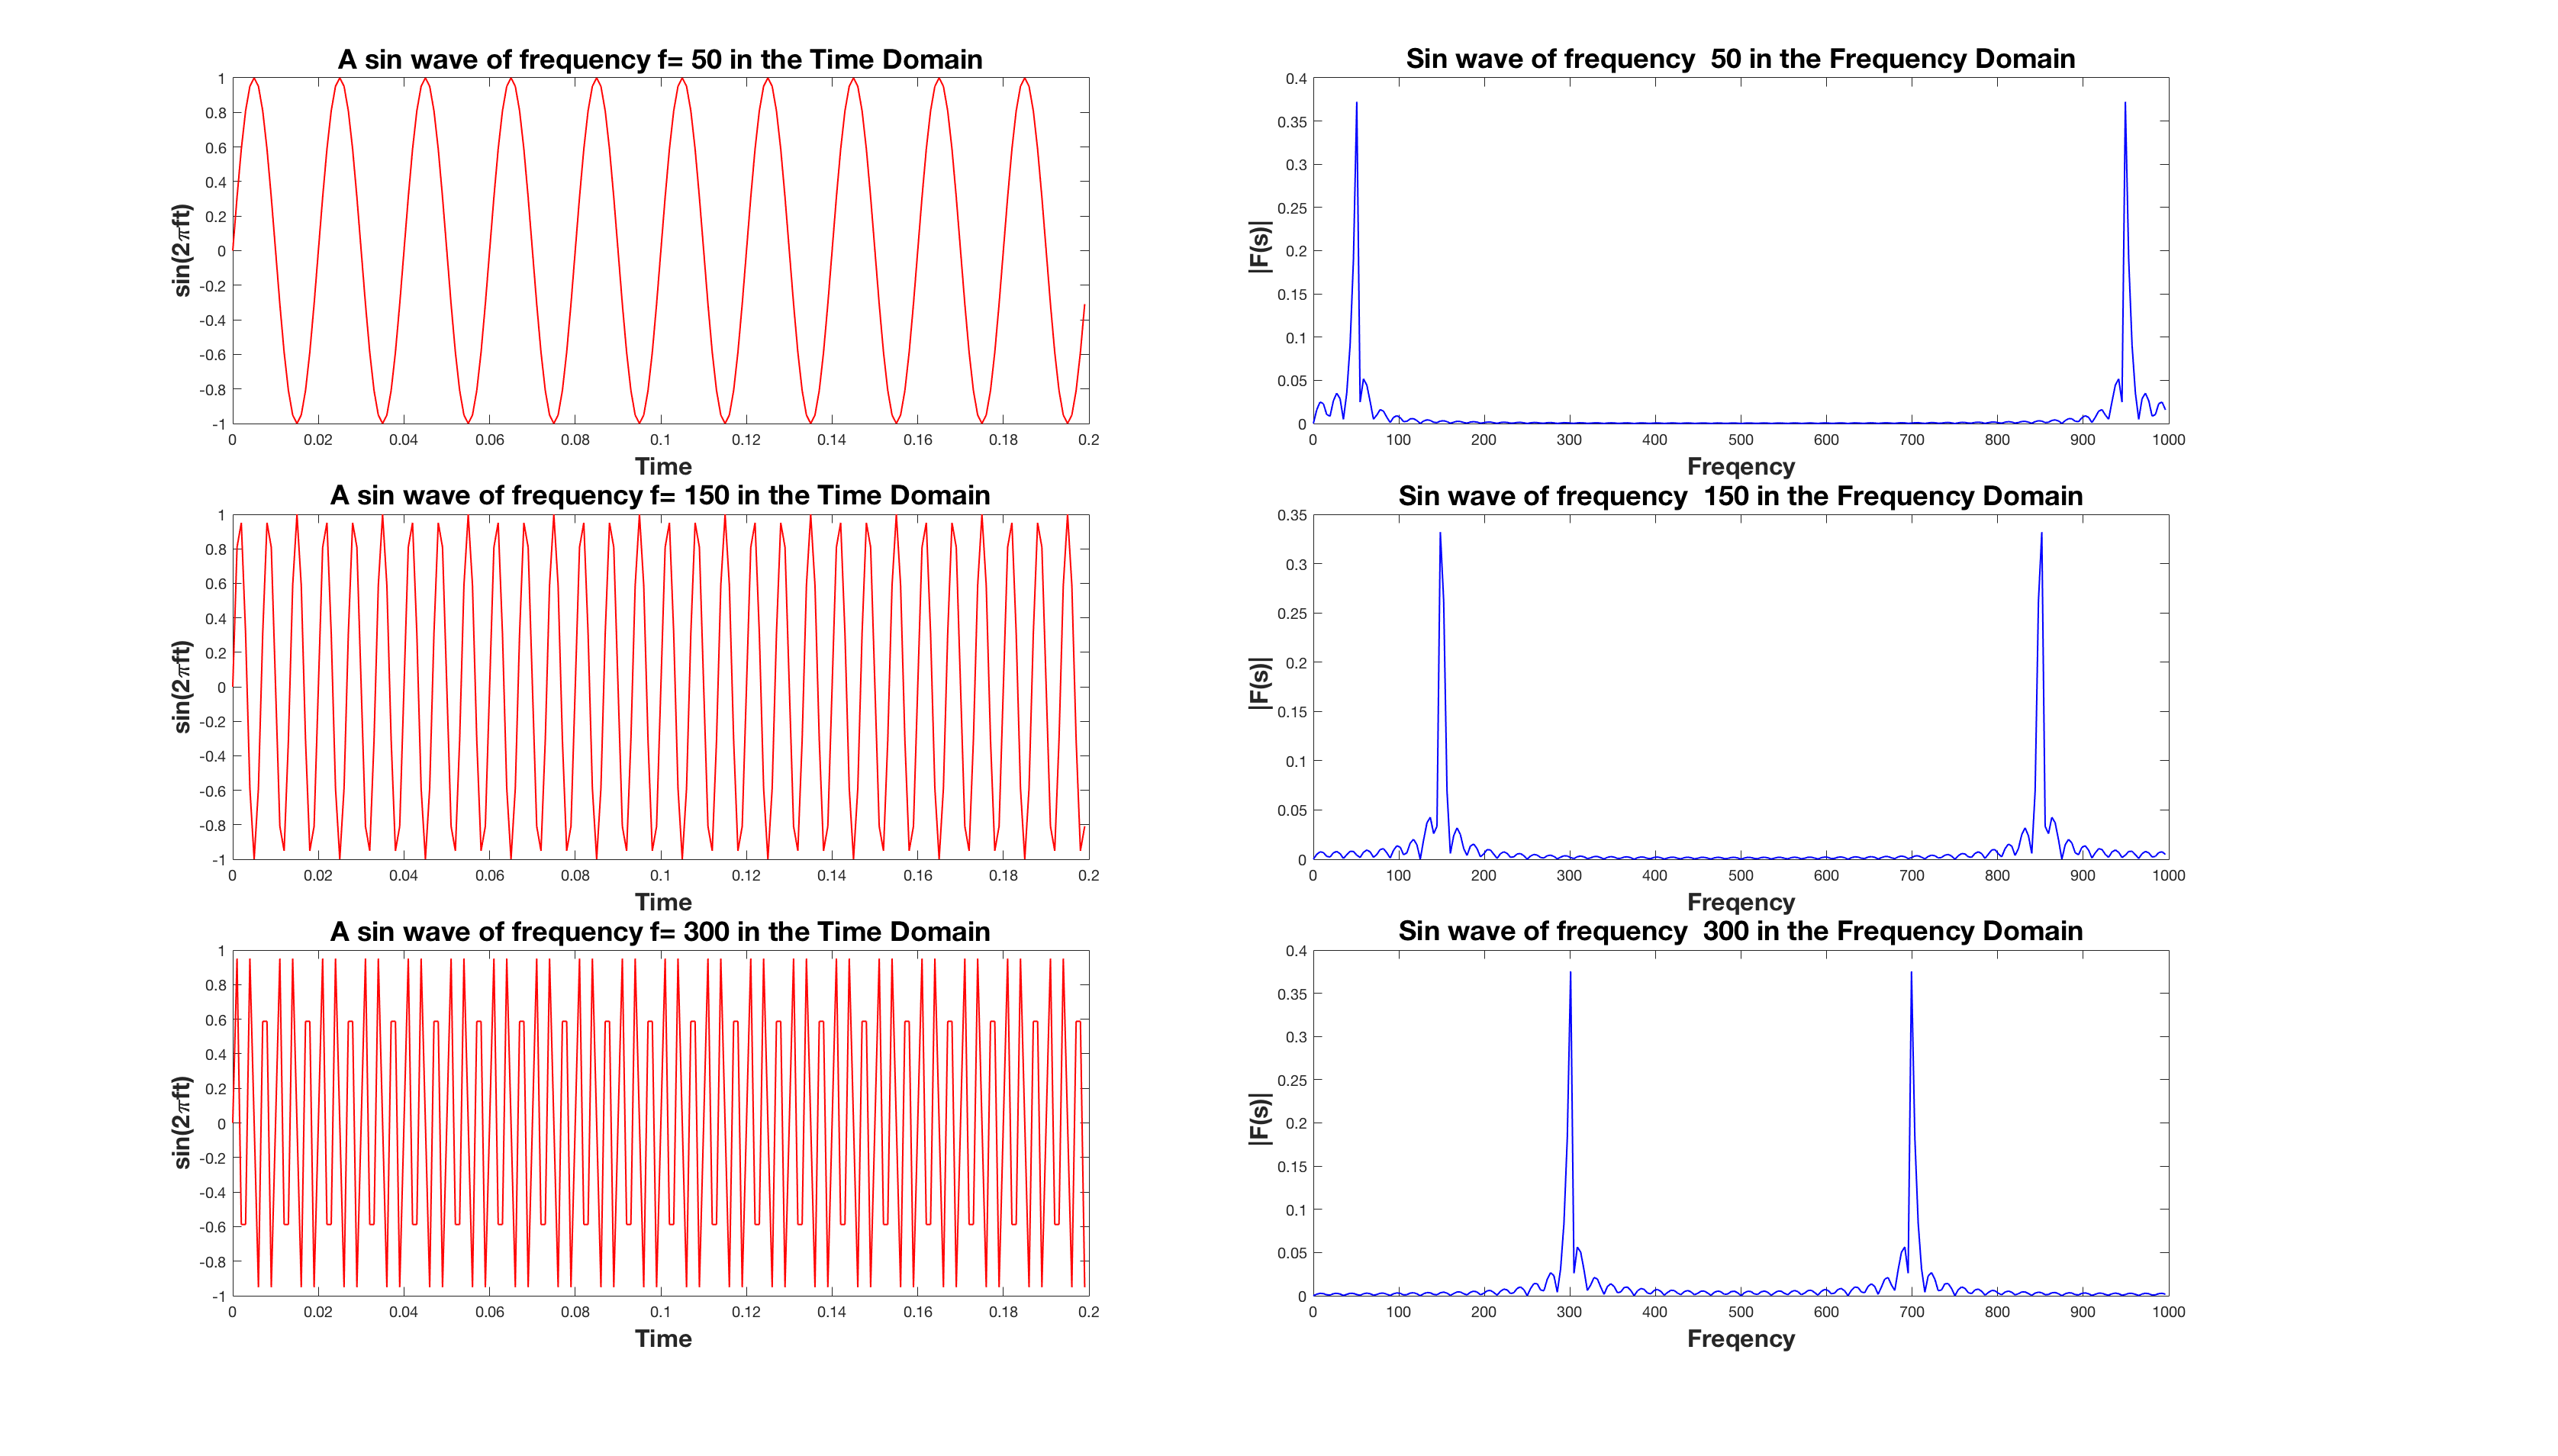
\includegraphics[scale=.15]{Images/fourier-sin}
\caption{Fourier Transforms for discretized time signal sine waves with three different frequencies and respective discrete Fourier transforms are given above. The sampling period used is 0.001 and total length of signal (L) is 200. The graphs were created using Matlab code DrawSinFourierGraph.m and it is attached in the Appendix B}
\label{fig:Fourier-sin}
\end{figure}

In the figure \ref{fig:Fourier-sin}, a sine wave with different frequencies ${f = 50,150,300}$ is transformed into the frequency domain using the discrete Fourier transform. Please note high amplitude in the frequency domain for their respective frequency in each graph. $\omega = 2\pi f$.

\begin{equation}
f(t) = \sin(\omega t) 
\end{equation}
Three types of sine wave are created with frequencies ${f =50, 150,300}$. The Fourier transform of the $f(t)$ is given by
\begin{equation}
\begin{split}
F(s)  &= \int_{-\infty}^{\infty}{\sin(2\pi f t) e^{-j2\pi t s }dt} \\
 \int_{-\infty}^{\infty}{\sin(2\pi f t) e^{-j2\pi t s }dt}  &= \frac{\delta(t-2\pi f) - \delta(t+2\pi f)}{2j}
 \end{split}
\end{equation}
Where $\delta(s)$ is the Dirac Delta function. The Dirac Delta function is defined as
$$
\delta(t) = \left\{ \begin{array}{rl}
 +\infty  &\mbox{ if $t=0$} \\
   0 &\mbox{ if $t\ne0$}
          \end{array} \right.
		  $$
\begin{equation}
\int_{-\infty}^{\infty} \delta(t) dt = 1 
\end{equation}
It follows that
\begin{equation}
\int_{-\infty}^{\infty} a \delta(t) dt = a 
\end{equation}
where a is a constant. 

For a function $f(t)$, being integrable, we have that
\begin{equation}
\int_{-\infty}^{\infty}  f(t) \delta(t) dt = f(0)
\end{equation}
It denotes that the integral of any function multiplied by a $\delta$-function located about zero is just the value of the function at zero. This concept can be extended to give the shifting property, again for a function $f(t)$, giving, 
\begin{equation}
\int_{-\infty}^{\infty}  f(t) \delta(t-a) dt = f(a)
\end{equation}
where $\delta(t-a)$ is just a $\delta$-function located at $t = a$. 
In two dimensions, for a function $f(t,w)$, we have that,
\begin{equation}
\int\int  f(t,w) \delta(t-a,w-b) dt dw = f(a,b)
\end{equation}
where $\delta(t-a,w-b)$ is a $\delta$-function located at position $a,b$. This property is central to the idea of convolution, which is used extensively in image formation theory, and in digital image processing. 
The Fourier transform of a $\delta$ function can be formed by direct integration using the definition of the Fourier transform, and the shift property. We get, 

\begin{equation} \label{eq:delta1}
\begin{split}
F(\delta(t)) & = \int_{-\infty}^{\infty} \delta(t) e^{-j2\pi s t} dt \\
 & = e^0 \\
 & = 1
 \end{split}
\end{equation}

\subsection{Shifting Theorem}
Let $f(t)$ be a function and its Fourier transform is given by $F(s)$. Fourier transform of a function $f(t-t_0)$ is given $e^{-j2\pi s t_0}F(s)$. The proof of the shift theorem is given below. $F[f(t-t_0)](s) = e^{-j 2 \pi s t_0} F(s)$

\begin{equation} 
F[f(t-t_0)](s) = \int_{-\infty}^{\infty} f(t-t_0)  e^{-j2\pi s t} dt 
\end{equation}
Multiply $e^{j2\pi s t_0} e^{-j2\pi s t_0} $ on right hand side of the above equation.
\begin{equation} 
\begin{split}
F[f(t-t_0)](s) &= \int_{-\infty}^{\infty} f(t-t_0) e^{-j2\pi s t} e^{j2\pi s t_0}  e^{-j2\pi s t_0} dt \\
& = e^{-j2\pi s t_0}  \int_{-\infty}^{\infty} f(t-t_0) e^{-j2\pi s (t-t_0)} dt 
 \end{split}
\end{equation}
Let $u = t-t_0$
\begin{equation} 
\begin{split}
F[f(t-t_0)](s) &= \int_{-\infty}^{\infty} f(u) e^{-j2\pi s u} du \\
& = e^{-j2\pi s t_0}  F(s)
 \end{split}
\end{equation}

By applying the shifting theorem in the equation \ref{eq:delta1},we get that, 
\begin{equation}
F(\delta(t-a)) = e^{-j2\pi s a}
\end{equation}
so that the Fourier transform of a shifted $\delta$ function is given by a phase ramp. The modulus squared of above equation is
\begin{equation}
\begin{split}
|F(\delta(t-a))|^2 & = |e^{-j2\pi s a}|^2 \\
& = 1
\end{split}
\end{equation}
The power spectrum of a $\delta$ function is constant independent of its location in real space. Noting that the Fourier transform is a linear operator, consider two $\delta$ functions located at $\pm a$. Then the Fourier transform of $\delta(t-a)+\delta(t+a)$ is given by
\begin{equation}
\begin{split}
F(\delta(t-a)+\delta(t+a)) & = e^{-j2\pi as}+e^{j2\pi as}\\
& = 2\cos(2 \pi as) \\
\int_{-\infty}^{\infty} \cos(2 \pi a t) e^{-j2\pi t s} &= \frac{\delta(t-a)+\delta(t+a)}{2}
\end{split}
\end{equation}
If we take the $\delta$-function at $t=-a$ as negative, the Fourier transform is given below
\begin{equation}
\begin{split}
F(\delta(t-a)-\delta(t+a)) & = e^{-j2\pi as}-e^{j2\pi as}\\
& = 2j\sin(2 \pi as) \\
\int_{-\infty}^{\infty} \sin(2 \pi a t) e^{-j2\pi t s} &= \frac{\delta(t-a)-\delta(t+a)}{2j}
\end{split}
\end{equation}
\begin{figure}[!ht]
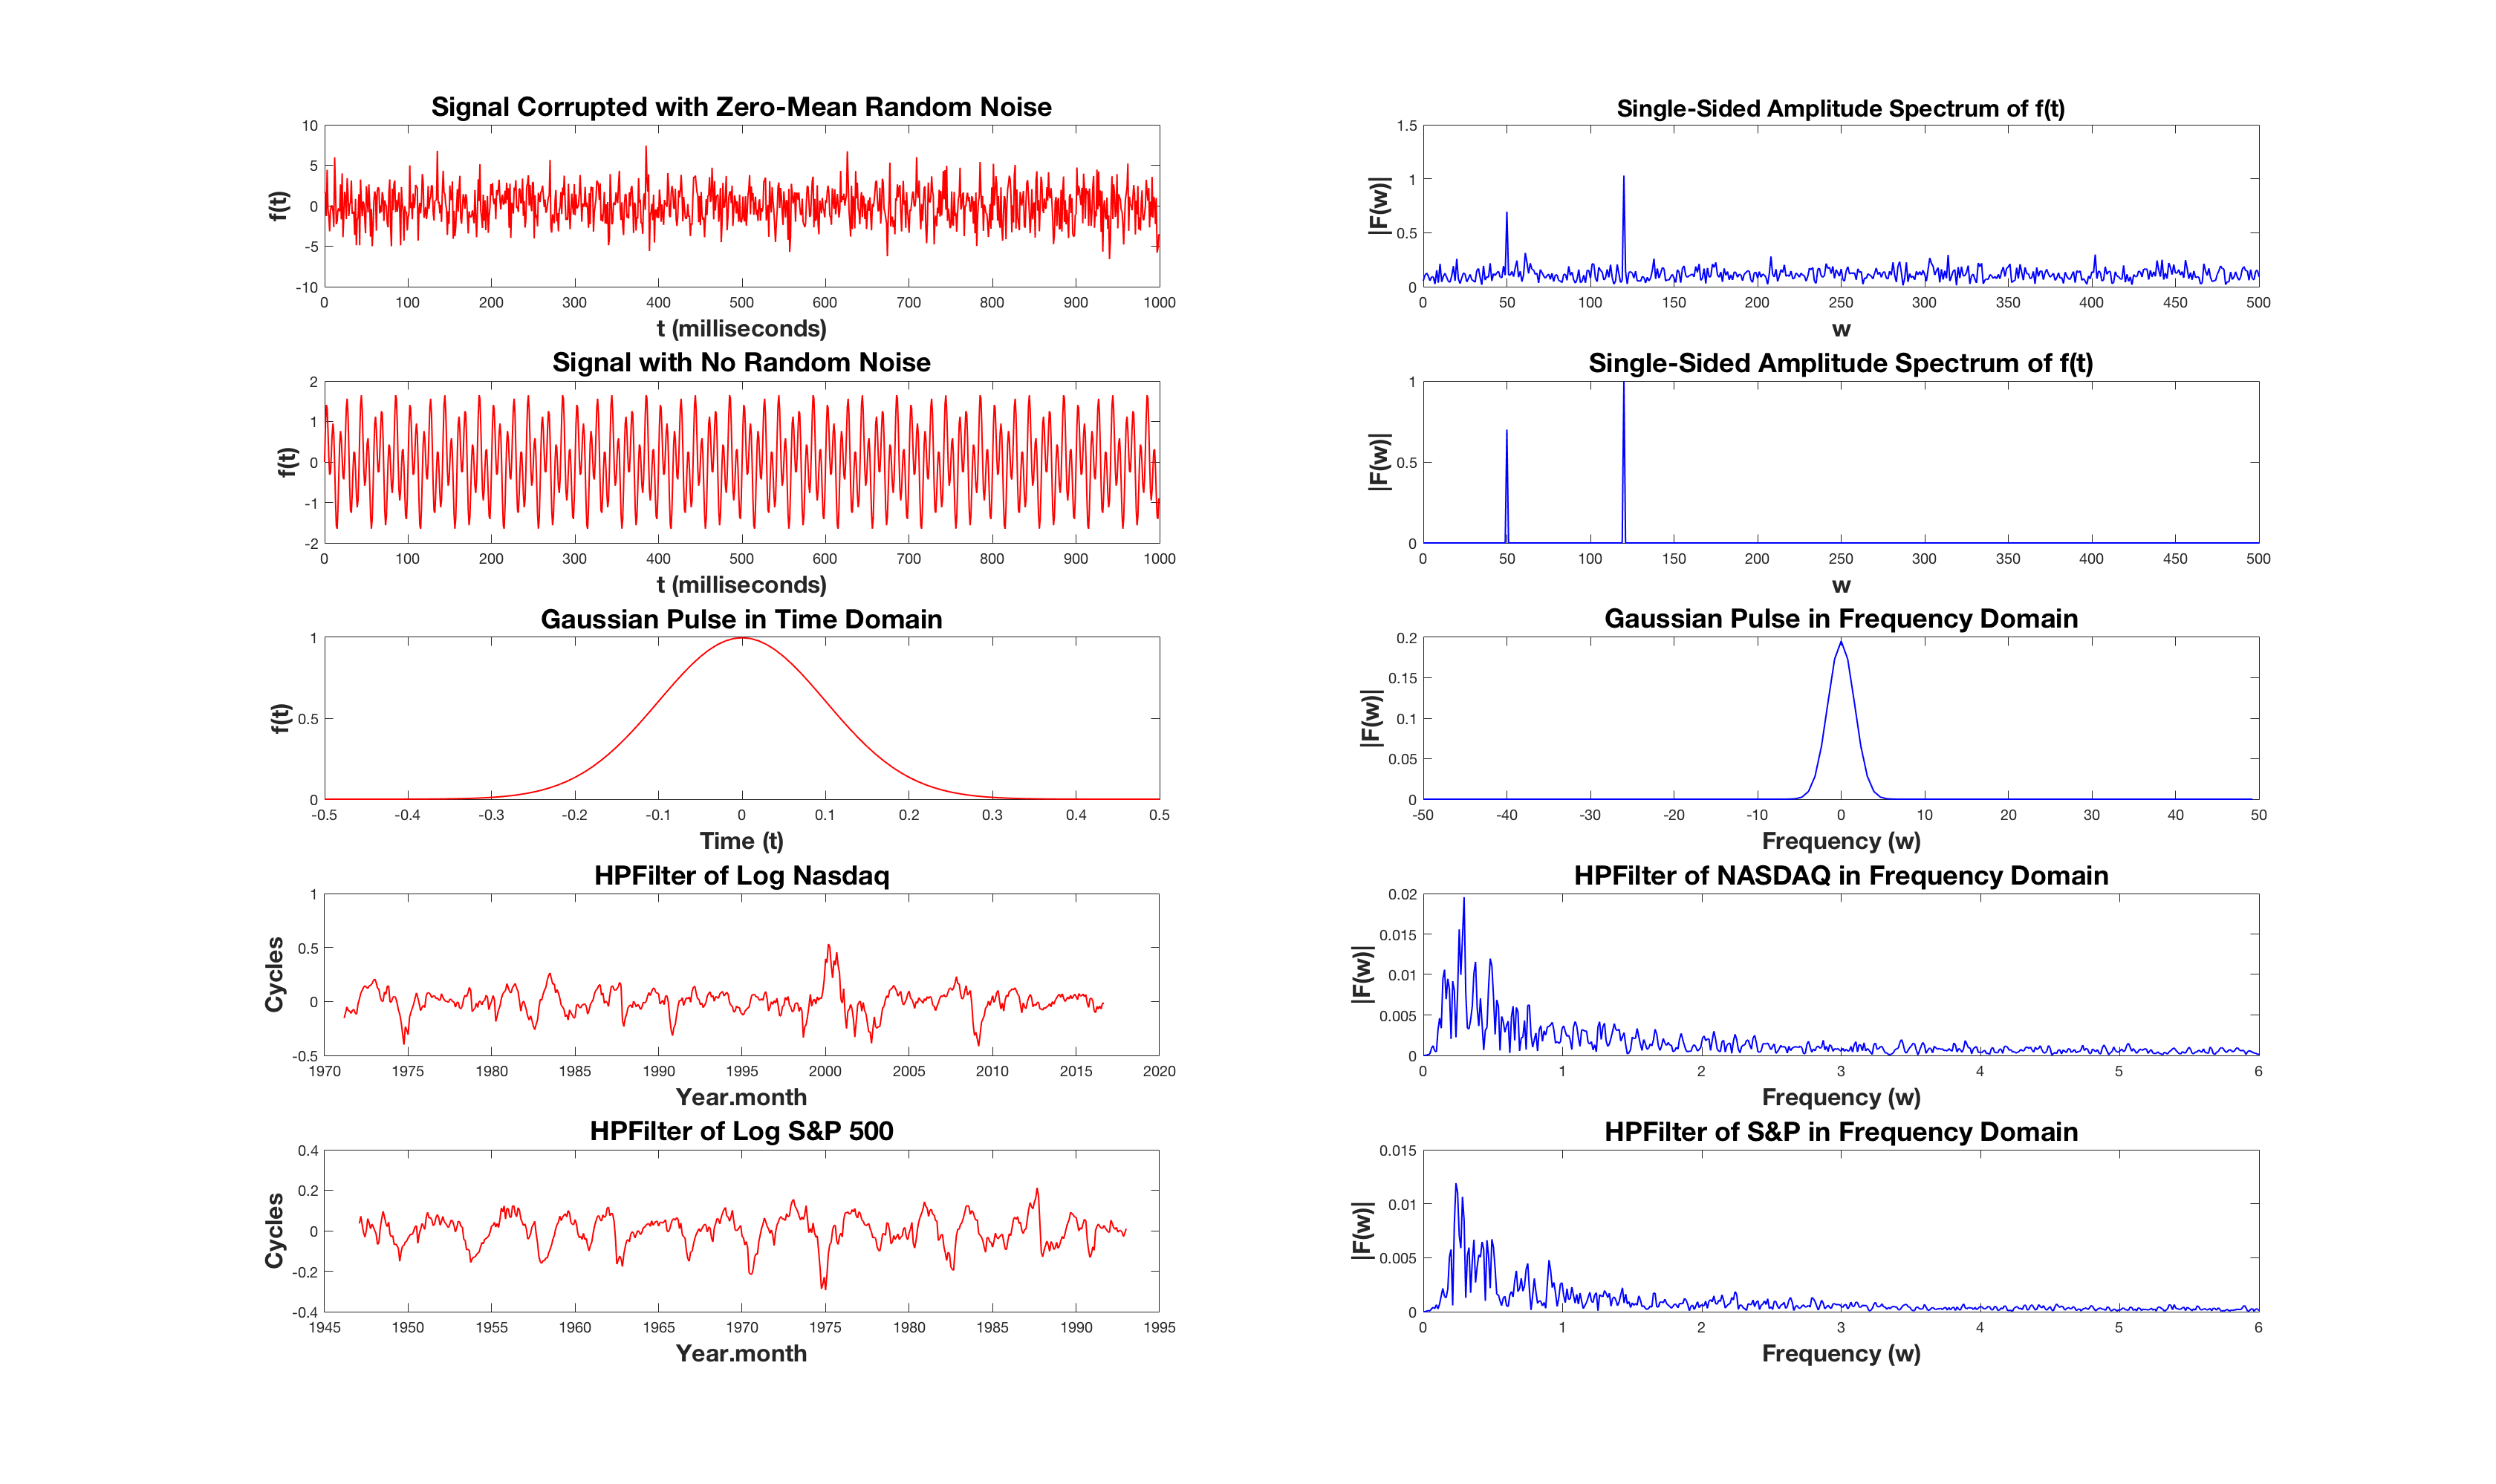
\includegraphics[scale=.15]{Images/fourier3}
\caption{Fourier transform for a) Zero mean signal with random noise, b) Zero mean signal $f(t) = 0.7sin(2\pi 50t)+sin(2\pi 120t)$, c) Gaussian - Frequency are shifted (using fftshift function in matlab) in the frequency domain to show that the Fourier transform of Gaussian looks like Gaussian in the frequency domain, d) HP Filter of Log NASDAQ, e) HP Filter of Log S\&P 500. The program used to generate the graph is SPNASDAQFourier.m and stored in Appendix }
\label{fig:Fourier3}
\end{figure}
In the figure \ref{fig:Fourier3}, a signal with zero mean random noise, signal with zero mean with no random noise, Gaussian curve, HP filter of $log$ sp500, HP filter of $log$ Nasdaq are also transformed into a  frequency domain using the discrete Fourier transform. $|F(s)|$ is an even function and so only $s>0$ is shown in figure \ref{fig:Fourier3}.
\subsection{Discrete Fourier Transform}
The Discrete Fourier Transform (DFT) is the equivalent of the continuous Fourier Transform for signals known only at N instants separated by sample times T (i.e a finite sequence of data). Let $f(k)$ be a continuous signal and the $N$ samples be denoted by $f(0), f(1), f(2)... f(k),...,f(N-1)$. Each sample $f(k)$ is regarded as an impulse having area $f(k)$ and the integrand exists only at the sample points.
\begin{comment}
\begin{align}
F(j2\pi s) &= \int_{0}^{(N-1)T}{f(t)e^{-j2\pi ts}dt}; \\
&= f[0]e^{-j0} + f(1)e^{-j2\pi sT}+...+f(k)e^{-j2\pi skT}+....f(N-1)e^{-j2\pi(N-1)T} \\
&= \sum_{k=0}^{N-1} f(k) e^{-j2\pi sk T}
\end{align}
\end{comment}
Since there are only a finite number of input data points, the DFT treats the data as if it were periodic i.e $f(N)$ to $f(2N-1)$ is the same as $f(0)$ to $f(N-1)$. In general, the discrete Fourier Transform is given by
\begin{equation}
F(s) = \sum_{k=0}^{N-1} f(k) e^{-j\frac{2\pi}{N} sk }
\end{equation}
$s = 0,1,..,N-1$.
\begin{equation}
e^{j\frac{2\pi}{N}} = \cos(\frac{2\pi}{N}) + j \sin(\frac{2\pi}{N})
\end{equation}
is the principal N-th root of unity. Since $ e^{j\frac{2\pi s}{N}}$ has a period of N, the DFT coefficients $F(s)$ are periodic with period N when $s$ is taken outside the range $s = 0,1,2,...N-1$. $F(s)$ is the Discrete Fourier Transform of the sequence $f(t)$. The matrix-vector format of the Discrete Fourier Transform are given by

$\underbrace{
\begin{bmatrix}
F(0) \\
F(1) \\
F(2) \\
\vdots \\
\vdots \\
F(N-1)
\end{bmatrix} }_{\text{DFT Vector} }$ \qquad
=
$\underbrace{
\begin{bmatrix}
1 & 1 & \cdots & \cdots & 1 \\
1 & e^{-j(\frac{2\pi}{N})} & e^{-j(\frac{4\pi}{N})}\cdots & \cdots & e^{-j\frac{2(N-1)\pi}{N}} \\
1 & e^{-j(\frac{4\pi}{N})} & e^{-j(\frac{8\pi}{N})}\cdots & \cdots &  e^{-j\frac{4(N-1)\pi}{N}} \\
\vdots & & & \vdots \\
\vdots & & & \vdots \\
1 & e^{-j(\frac{2(N-1)\pi}{N})} & e^{-j(\frac{4(N-1)\pi}{N})}\cdots & \cdots & e^{-j\frac{2(N-1)(N-1)\pi}{N}} \\
\end{bmatrix} }_{\text{DFT Matrix:F}}$
$\underbrace{
\begin{bmatrix}
f(0) \\ f(1) \\ f(2) \\ \vdots \\ \vdots \\ f(N-1) 
\end{bmatrix}}_{\text{Input Signal}}$

The above matrix multiplication can also be used to compute the Discrete Fourier Transform of a given signal $f(t)$.  The Discrete Fourier Transform matrix F can be precomputed as it is independent of the input signal. 

\begin{figure}[!ht]
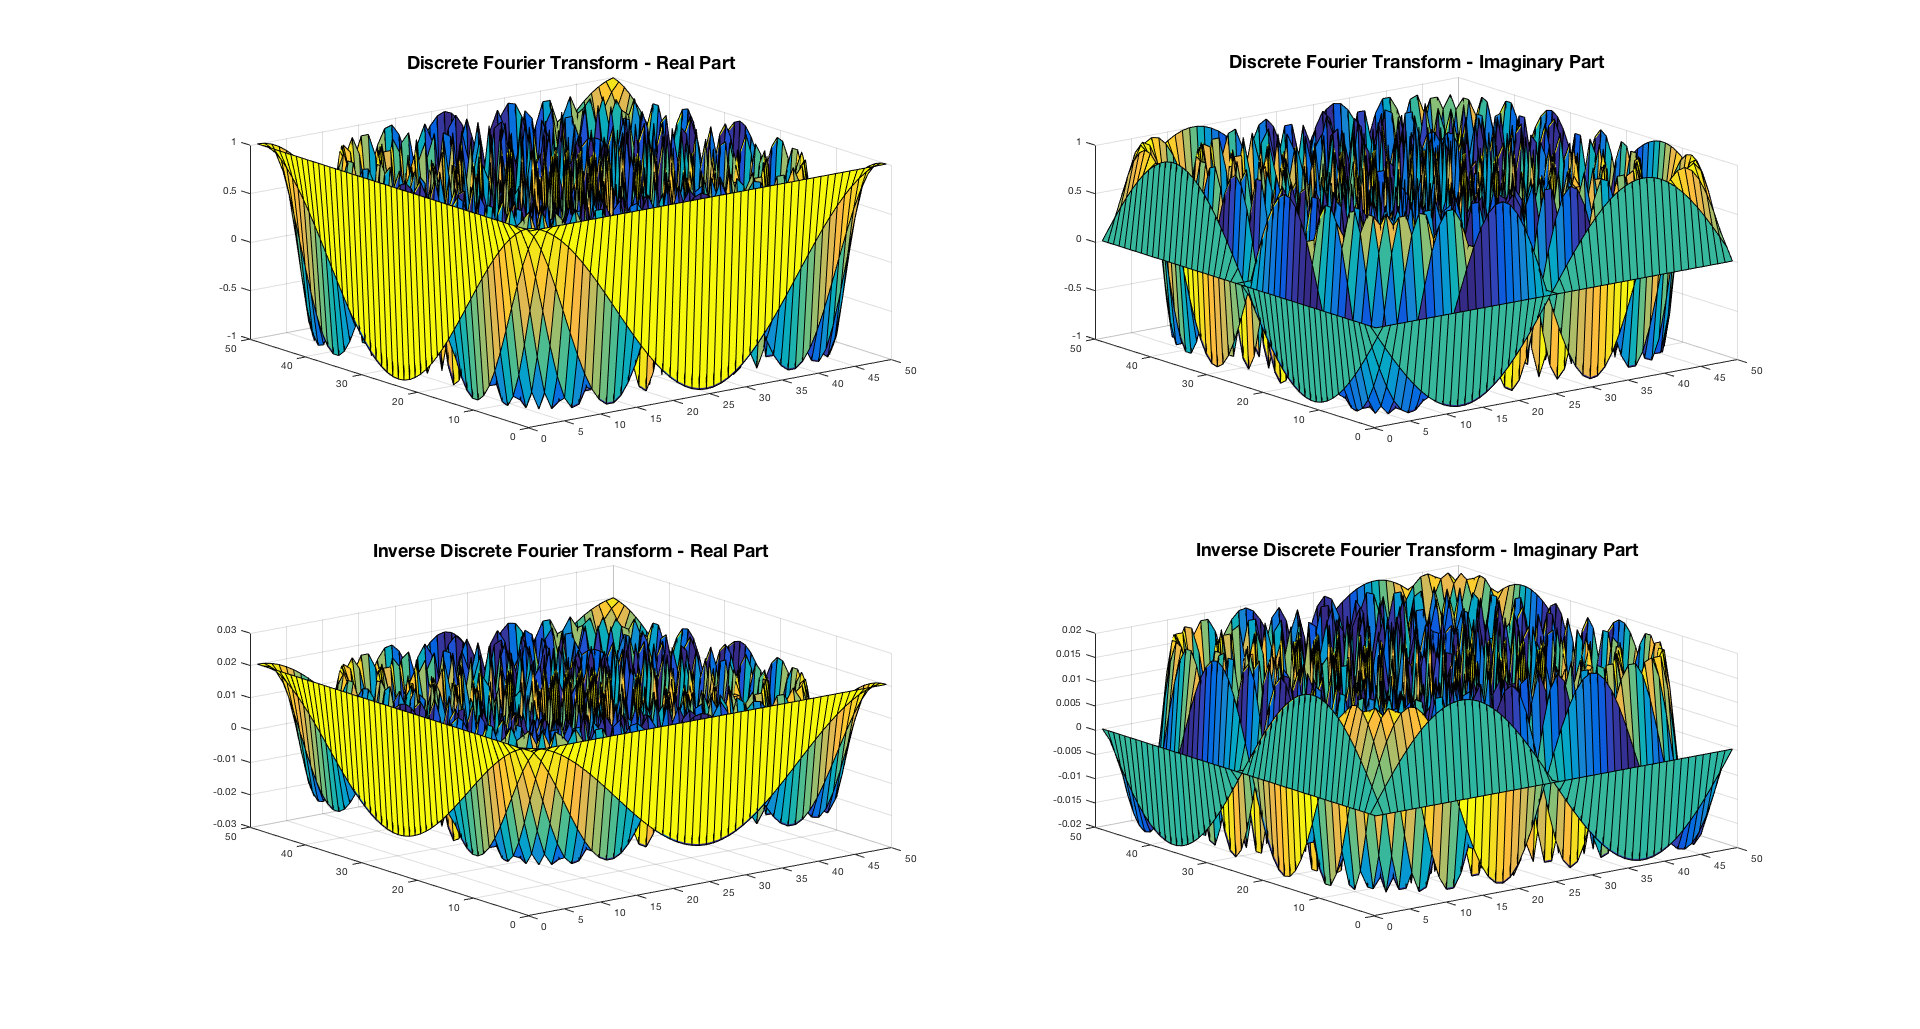
\includegraphics[scale=.22]{Images/DFTRANDI}
\caption{Discrete Fourier Transform \& Inverse DFT real and imaginary part. The above surface created using the matrix F. The graph is created using Matlab program named mydft.m attached in the Appendix}
\label{fig:DFTRANDI}
\end{figure}

\subsubsection{Inverse Discrete Fourier Transform}
The inverse transform of Discrete Fourier Transform is given by

\begin{equation}
f(t) = \frac{1}{N}\sum_{k=0}^{N-1} F(k) e^{j\frac{2\pi}{N} tk }
\end{equation}
The matrix-vector format of the Inverse Discrete Fourier Transform are given by

$\underbrace{
\begin{bmatrix}
f(0) \\
f(1) \\
f(2) \\
\vdots \\
\vdots \\
f(N-1)
\end{bmatrix}}_{\text{Original Signal}}$ \!
= $\frac{1}{N}$
$\underbrace{
\begin{bmatrix}
1 & 1 & \cdots & \cdots & 1 \\
1 & e^{j(\frac{2\pi}{N})} & e^{j(\frac{4\pi}{N})}\cdots & \cdots & e^{j(\frac{2(N-1)\pi}{N}} \\
1 & e^{j(\frac{4\pi}{N})} & e^{j(\frac{8\pi}{N})}\cdots & \cdots &  e^{j(\frac{4(N-1)\pi}{N}} \\
\vdots & & & \vdots \\
\vdots & & & \vdots \\
1 & e^{j(\frac{2(N-1)\pi}{N})} & e^{j(\frac{4(N-1)\pi}{N})}\cdots & \cdots & e^{j(\frac{2(N-1)(N-1)\pi}{N}}) \\
\end{bmatrix} }_{\text{Inverse DFT Matrix:G}}$
$\underbrace{
\begin{bmatrix}
F(0) \\ F(1) \\ F(2) \\ \vdots \\ \vdots \\ F(N-1) 
\end{bmatrix}}_{\text{DFT Vector}}$

The inverse DFT matrix G is inverse of matrix F and scaled by a factor of $\frac{1}{N}$. $G * F = F * G = I$, where as I is an identify matrix of order N. 

\subsection{Short Time Fourier Transformation}
 One of the ideas is to chop the signal into smaller pieces and perform Fourier transformation for each piece. This technique is called short time Fourier Transform. The smaller pieces in the signal can be chosen by a window function $w(t-\tau)$
 \begin{equation}
F(\tau,s) = \int_{-\infty}^{\infty}{f(t)w(t-\tau)e^{-j2\pi t s }dt}
\end{equation}
$w(t)$ represents a window function and there are multiple window functions available to choose. 

\subsubsection{Gaussian Window}
The Gaussian Window is defined as 
\begin{equation}
w(n) = e^\frac{-(n-m)^2}{2(\sigma N)^2}
\end{equation}
for $n = 0,1,2,... N-1$,where $N$ is the length of the window, $m=\frac{(N-1)}{2.0}$, and the $\sigma$ is the standard deviation of the Gaussian window. The Gaussian window is useful for time-frequency analysis because the Fourier transform and the derivate of a Gaussian window both are Gaussian function.

\subsubsection{Hamming Window}
The Hamming window is defined as 
 \begin{equation}
w(n) = \alpha - \beta \cos(\frac{2\pi n}{N - 1})
\end{equation}
where the constants $\alpha$ and $\beta$ are approximations to the values of $\frac{25}{46}$ and $\frac{21}{46}$ respectively. The values of $\alpha$ and $\beta$ are given as $0.54$ and $0.46$ respectively. 

 \begin{equation}
w(n) = 0.54 - 0.46 \cos(\frac{2\pi n}{N - 1}), 0 \le n \le N
\end{equation}
The window length is $L = N + 1$.

\begin{figure}[!ht]
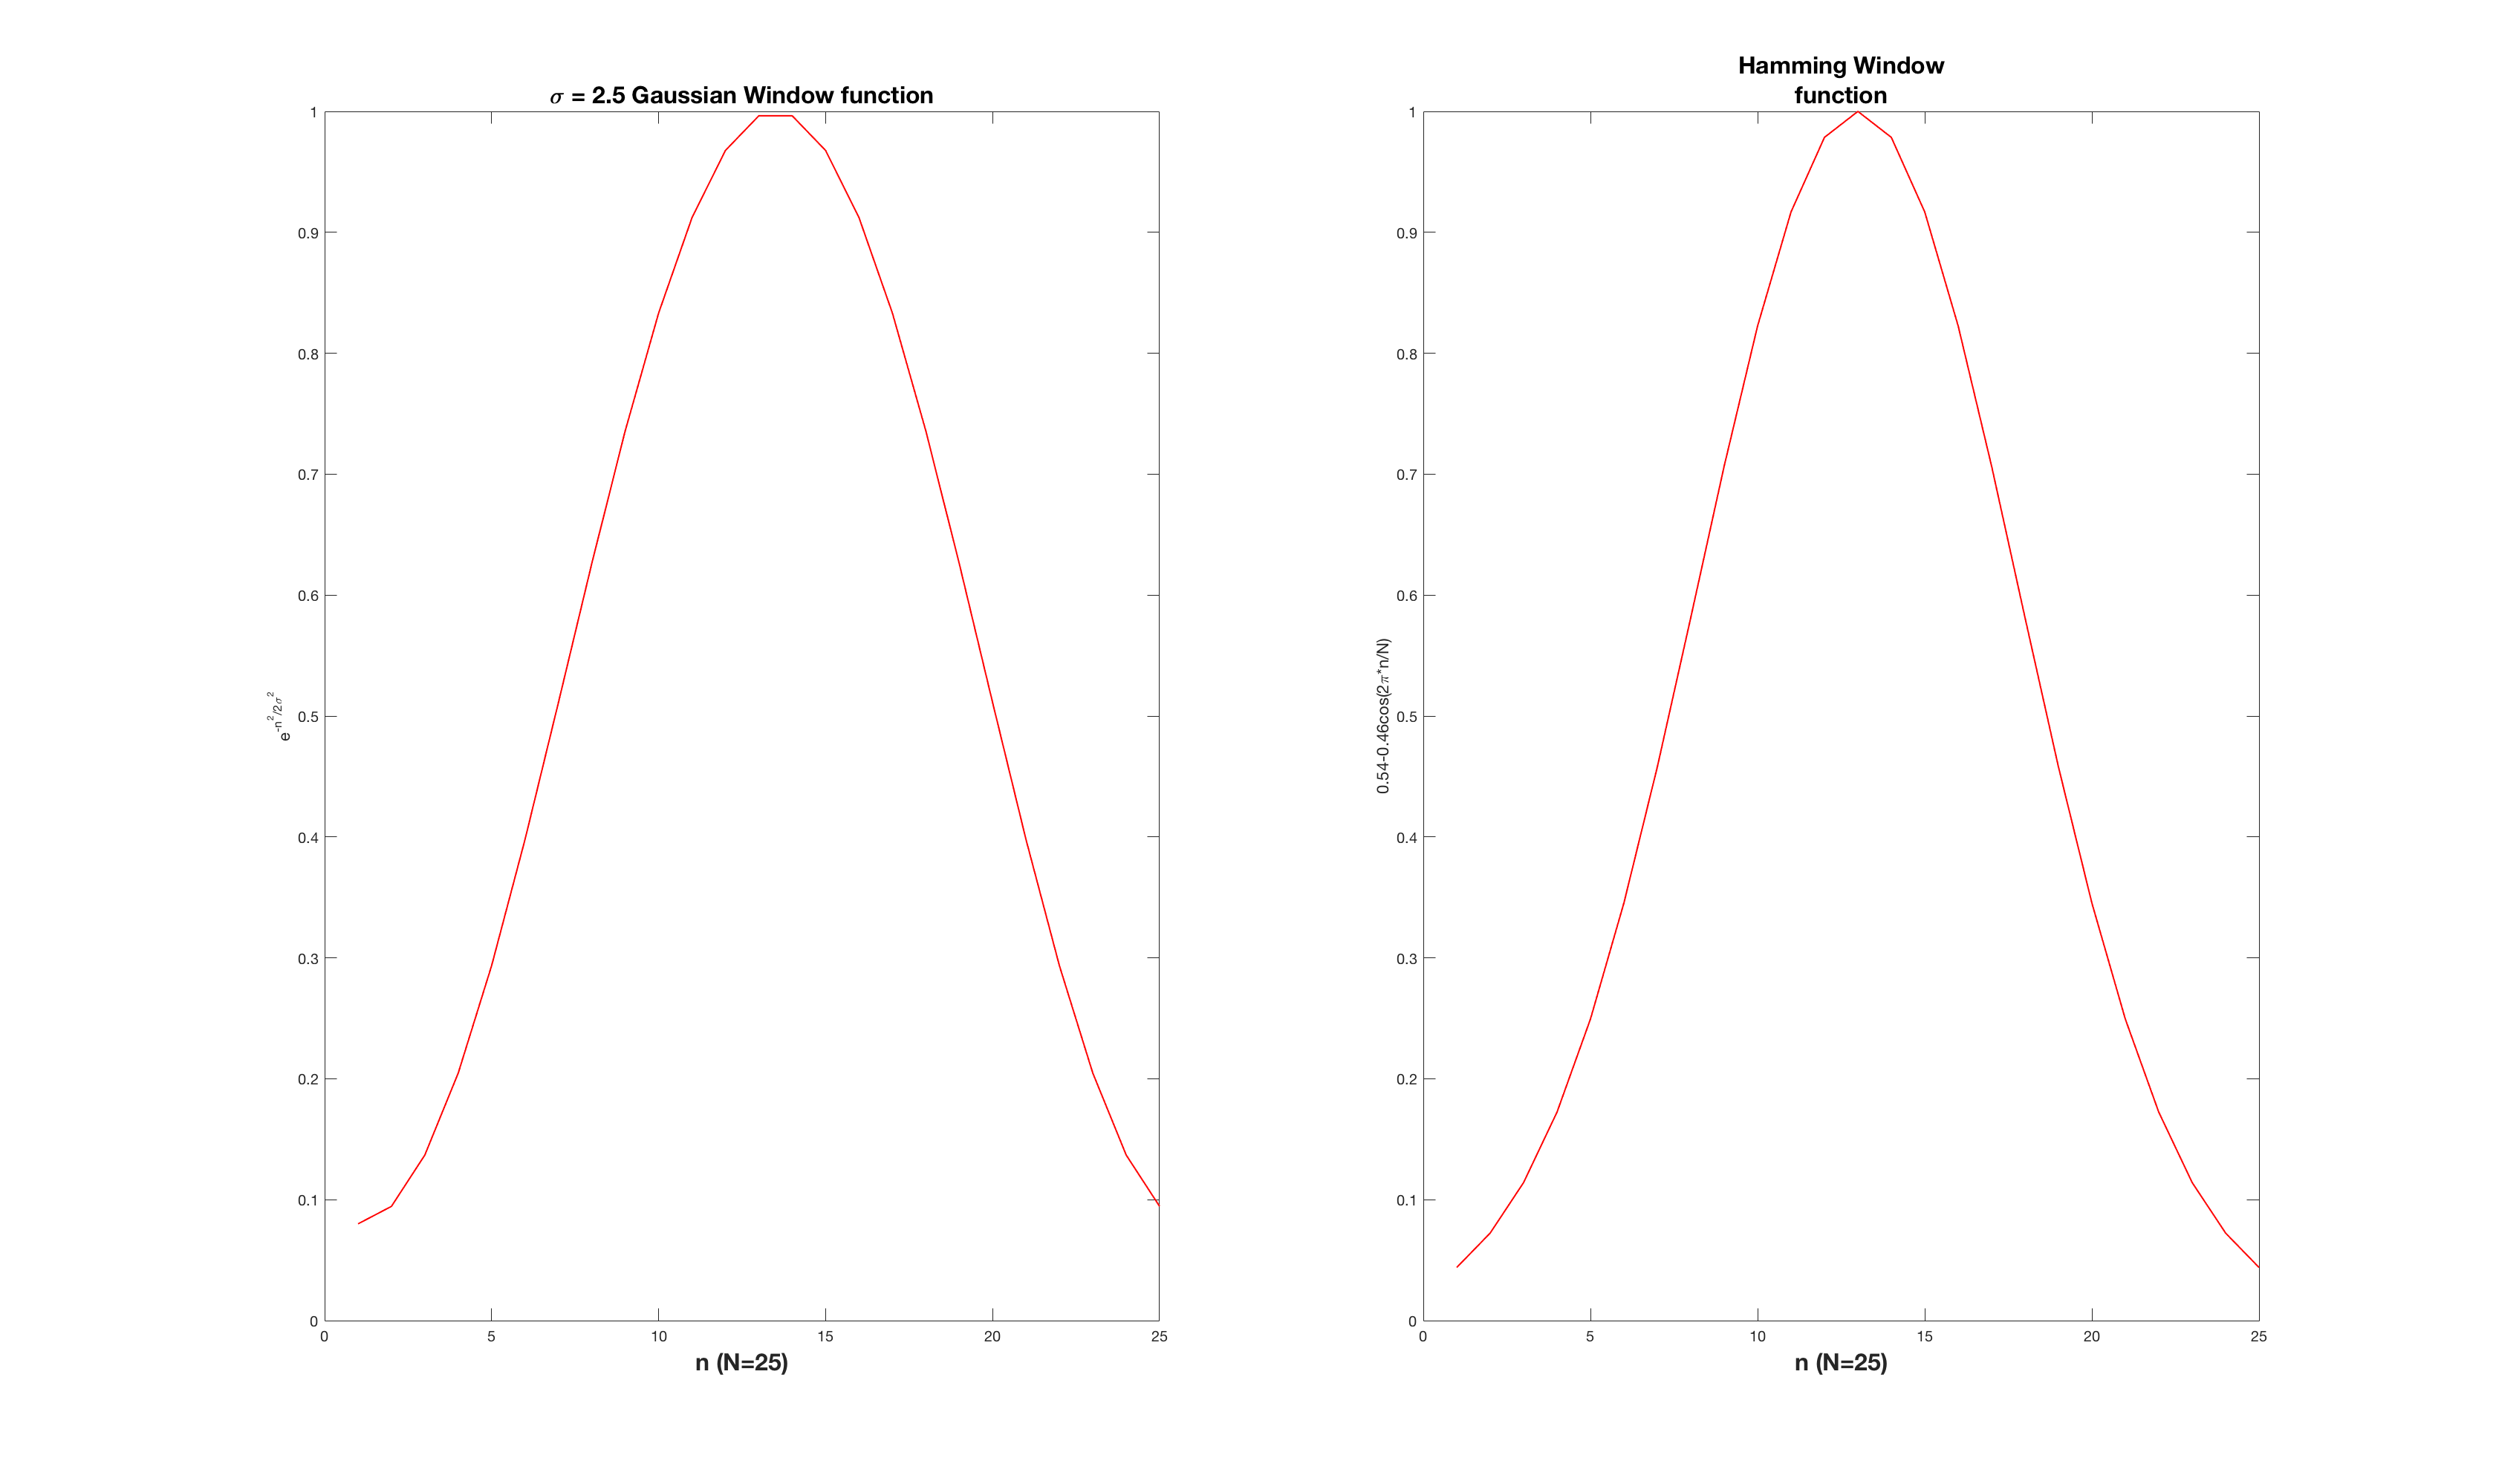
\includegraphics[scale=.15]{Images/GWinHWin}
\caption{Window function (window length  =25) for a) Gaussian b) Hamming. The graph was created using Matlab program ghamwin.m and attached in Appendix B }
\label{fig:ghamwin}
\end{figure}

The short time Fourier transform is performed for several signals using Hamming and Gaussian windows and the results are given below.

The first signal is

\begin{equation}\label{pwise}
f(t)  =
\left\{
\!
\begin{aligned}
sin(2\pi 300 t)  & \quad \quad \text{ if }\quad 0< t<\frac{T}{3}\\
sin(2\pi 200 t)  & \quad \quad \text{ if }\quad \frac{T}{3}+1<t<\frac{2T}{3}\\
sin(2\pi 100 t)  & \quad \quad \text{ if }\quad  \frac{2T}{3}+1<t<T
\end{aligned}
\right.
\end{equation}
Where T is the complete duration of $f(t)$. Operations like Fourier Transformation, Short Time Fourier Transform (STFT), STFT with Gaussian and Hamming windows are performed for the function given in \ref{pwise} and results of it is compared with similar operations for the SP500 Cycles, NASDAQ Cycles and results are given in Figure \ref{pwise}

\begin{figure}[!ht]
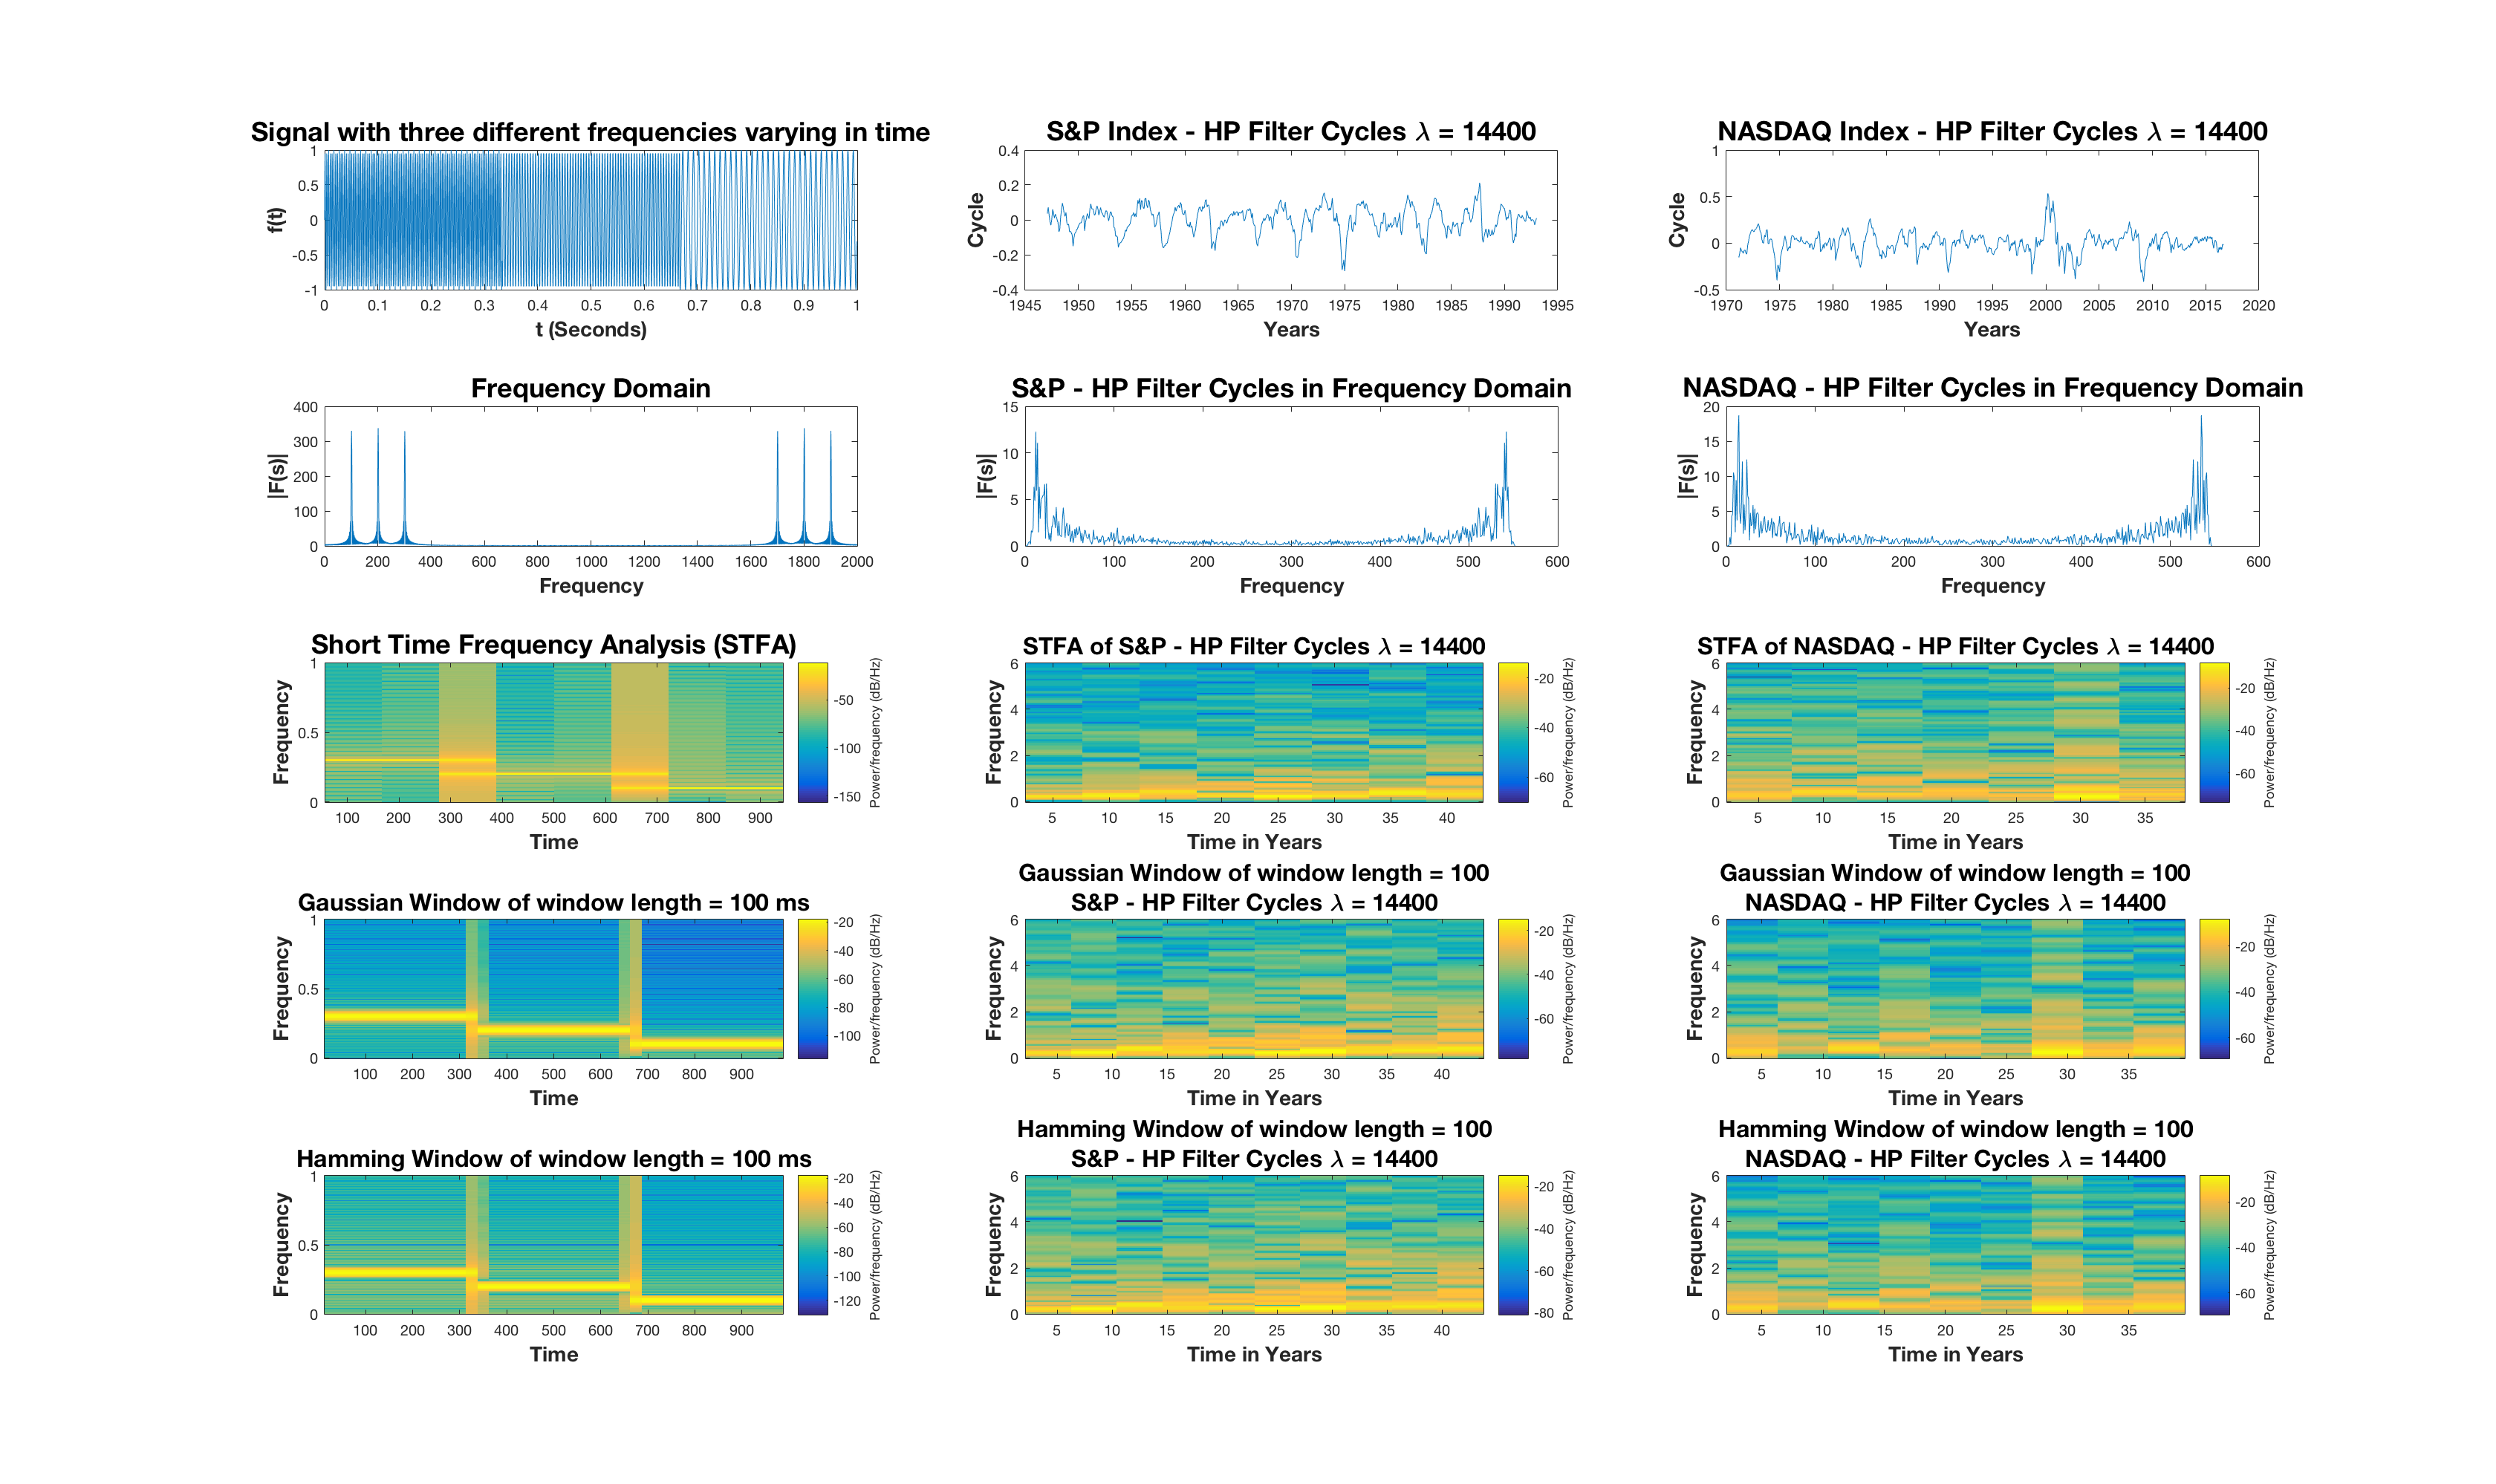
\includegraphics[scale=.16]{Images/Spectrum}
\caption{In the first column, the signal $f(t)$ as defined in \ref{pwise} b) Fourier Transform of $f(t)$ c) Short Time Fourier Transform of $f(t)$ d) STFT using Gaussian window e) STFT using Hamming window. Second column is for SP500 and third column is for NASDAQ indexes. The graph was created using Matlab program spectrumAnalysis5.m and attached in Appendix B }
\label{fig:spectrum}
\end{figure}


Simultaneous analysis of signals in both time and frequency domains provides better understanding of the signal and the short time Fourier transform laid the foundation for the joint time-frequency analysis.
\section{Introduction to Gabor Transformation}
The Gabor transformation or expansion in signal synthesis uses the Gabor elementary function (GEF) as the base function (equivalent of simple harmonic function in the Fourier transform) and the idea was influenced by Heisenberg's uncertainty principle.  \\
\subsection{Heisenberg's uncertainty principle}
In quantum mechanics, simultaneously, both the position of a particle and the momentum of the particle can not be measured preciously. Let $x$ be position and $p$ be momentum of the particle. The standard deviation of $x$ and $p$ are denoted by $\Delta x$ and $\Delta p$ respectively. The uncertainty principle states that product of the standard deviations of position and momentum is greater than or equal to $\frac{\hbar}{2}$
\begin{equation*}
\Delta x\Delta p \geq \frac{\hbar}{2}
\end{equation*}
\begin{equation*}
\begin{split}
\Delta x &= \sqrt{\langle(x - \langle x\rangle)^2\rangle} \\
\Delta p &= \sqrt{\langle(p - \langle p \rangle)^2\rangle}
\end{split}
\end{equation*}

\begin{comment}
\begin{equation*}
\Delta p = \sqrt{\langle(p - \langle p \rangle)^2\rangle}
\end{equation*}
\end{comment}

\subsection{Gabor Transformation }
Gabor had the insight that the base function with minimum uncertainty in both time and frequency domains best captures temporal information during the frequency analysis.

Gabor in his original study proposed an elementary function in complex form which occupies minimum uncertainty and it is a product of harmonic oscillator of any frequency and a Gaussian function. The area occupied by the following elementary function in the joint time frequency domain is equal to the minimum uncertainty.

\begin{equation}
\zeta(t) = \underbrace{e^{-\alpha ^2(t)^2}}_v\overbrace{e^{j2\pi f_0 t+\phi}}^w
\end{equation}

An arbitrary function $f(t)$ can be represented by a series of elementary functions which are constructed by translation in both the time and frequency domains. The function $f(t)$ is synthesized by the combination of GEFs.\\

\begin{equation}\label{gcoff}
f(t) = \sum_{m,n\in Z} C_{m,n} \psi_{m,n}(t)
\end{equation}
where the $C_{m,n}$ are Gabor coefficients and the $\psi_{m,n}(t)$ are the bases functions called Gabor elementary functions. A GEF translated by 'na' is denoted by $\psi_n$ and given by
\begin{equation*}
\psi_{n}(t) = \psi(t-na)\\
\end{equation*}
The translation in the frequency domain is also called modulation. A GEF is modulated by using simple harmonic functions. 
\begin{equation*}
\psi_{m,n}(t) = \psi(t-ma) e^{j2\pi nbt}
\end{equation*}\\
The original Gabor paper suggested that $\psi$ is Gaussian. GEFs were studied by using other functions for $\psi$ like a rectangle.  a and b are time and frequency shift parameters and a,b $>$  0. $\psi_{m,n}$ is obtained by shifting it by  ma $\times$ nb in the time-frequency plane.\\

For the given data set of NASDAQ and SP500 indexes data, the shift is towards a discrete time signal that is sampled for a finite time. Recalling \ref{gcoff}, 
\begin{equation}\label{gcoff1}
f(t) = \sum_{m=0}^{M-1}\sum_{n=0}^{N-1} C_{m,n} \psi_{m,n}(t)
\end{equation}
where $\psi_{m,n}(t)$ is Gabor Elementary functions.
$C_{m,n}$ is calculated as follows
\begin{equation}\label{cmn}
C_{m,n}  = \sum_t f(t) h(t-m\Delta M) e^\frac{-j2\pi t n\Delta N}{N}
\end{equation}
where $h$ is an analysis window.
$\Delta M$, $\Delta N$ are time and frequency sampling intervals respectively. $M$, $N$ are the number of sampling points in time and frequency domains. $\Delta M$, $\Delta N$, $M$, $N$ are chosen to meet the sampling criteria, $M\Delta M = L$ and $N\Delta N = L$. 


\begin{figure}[!ht]
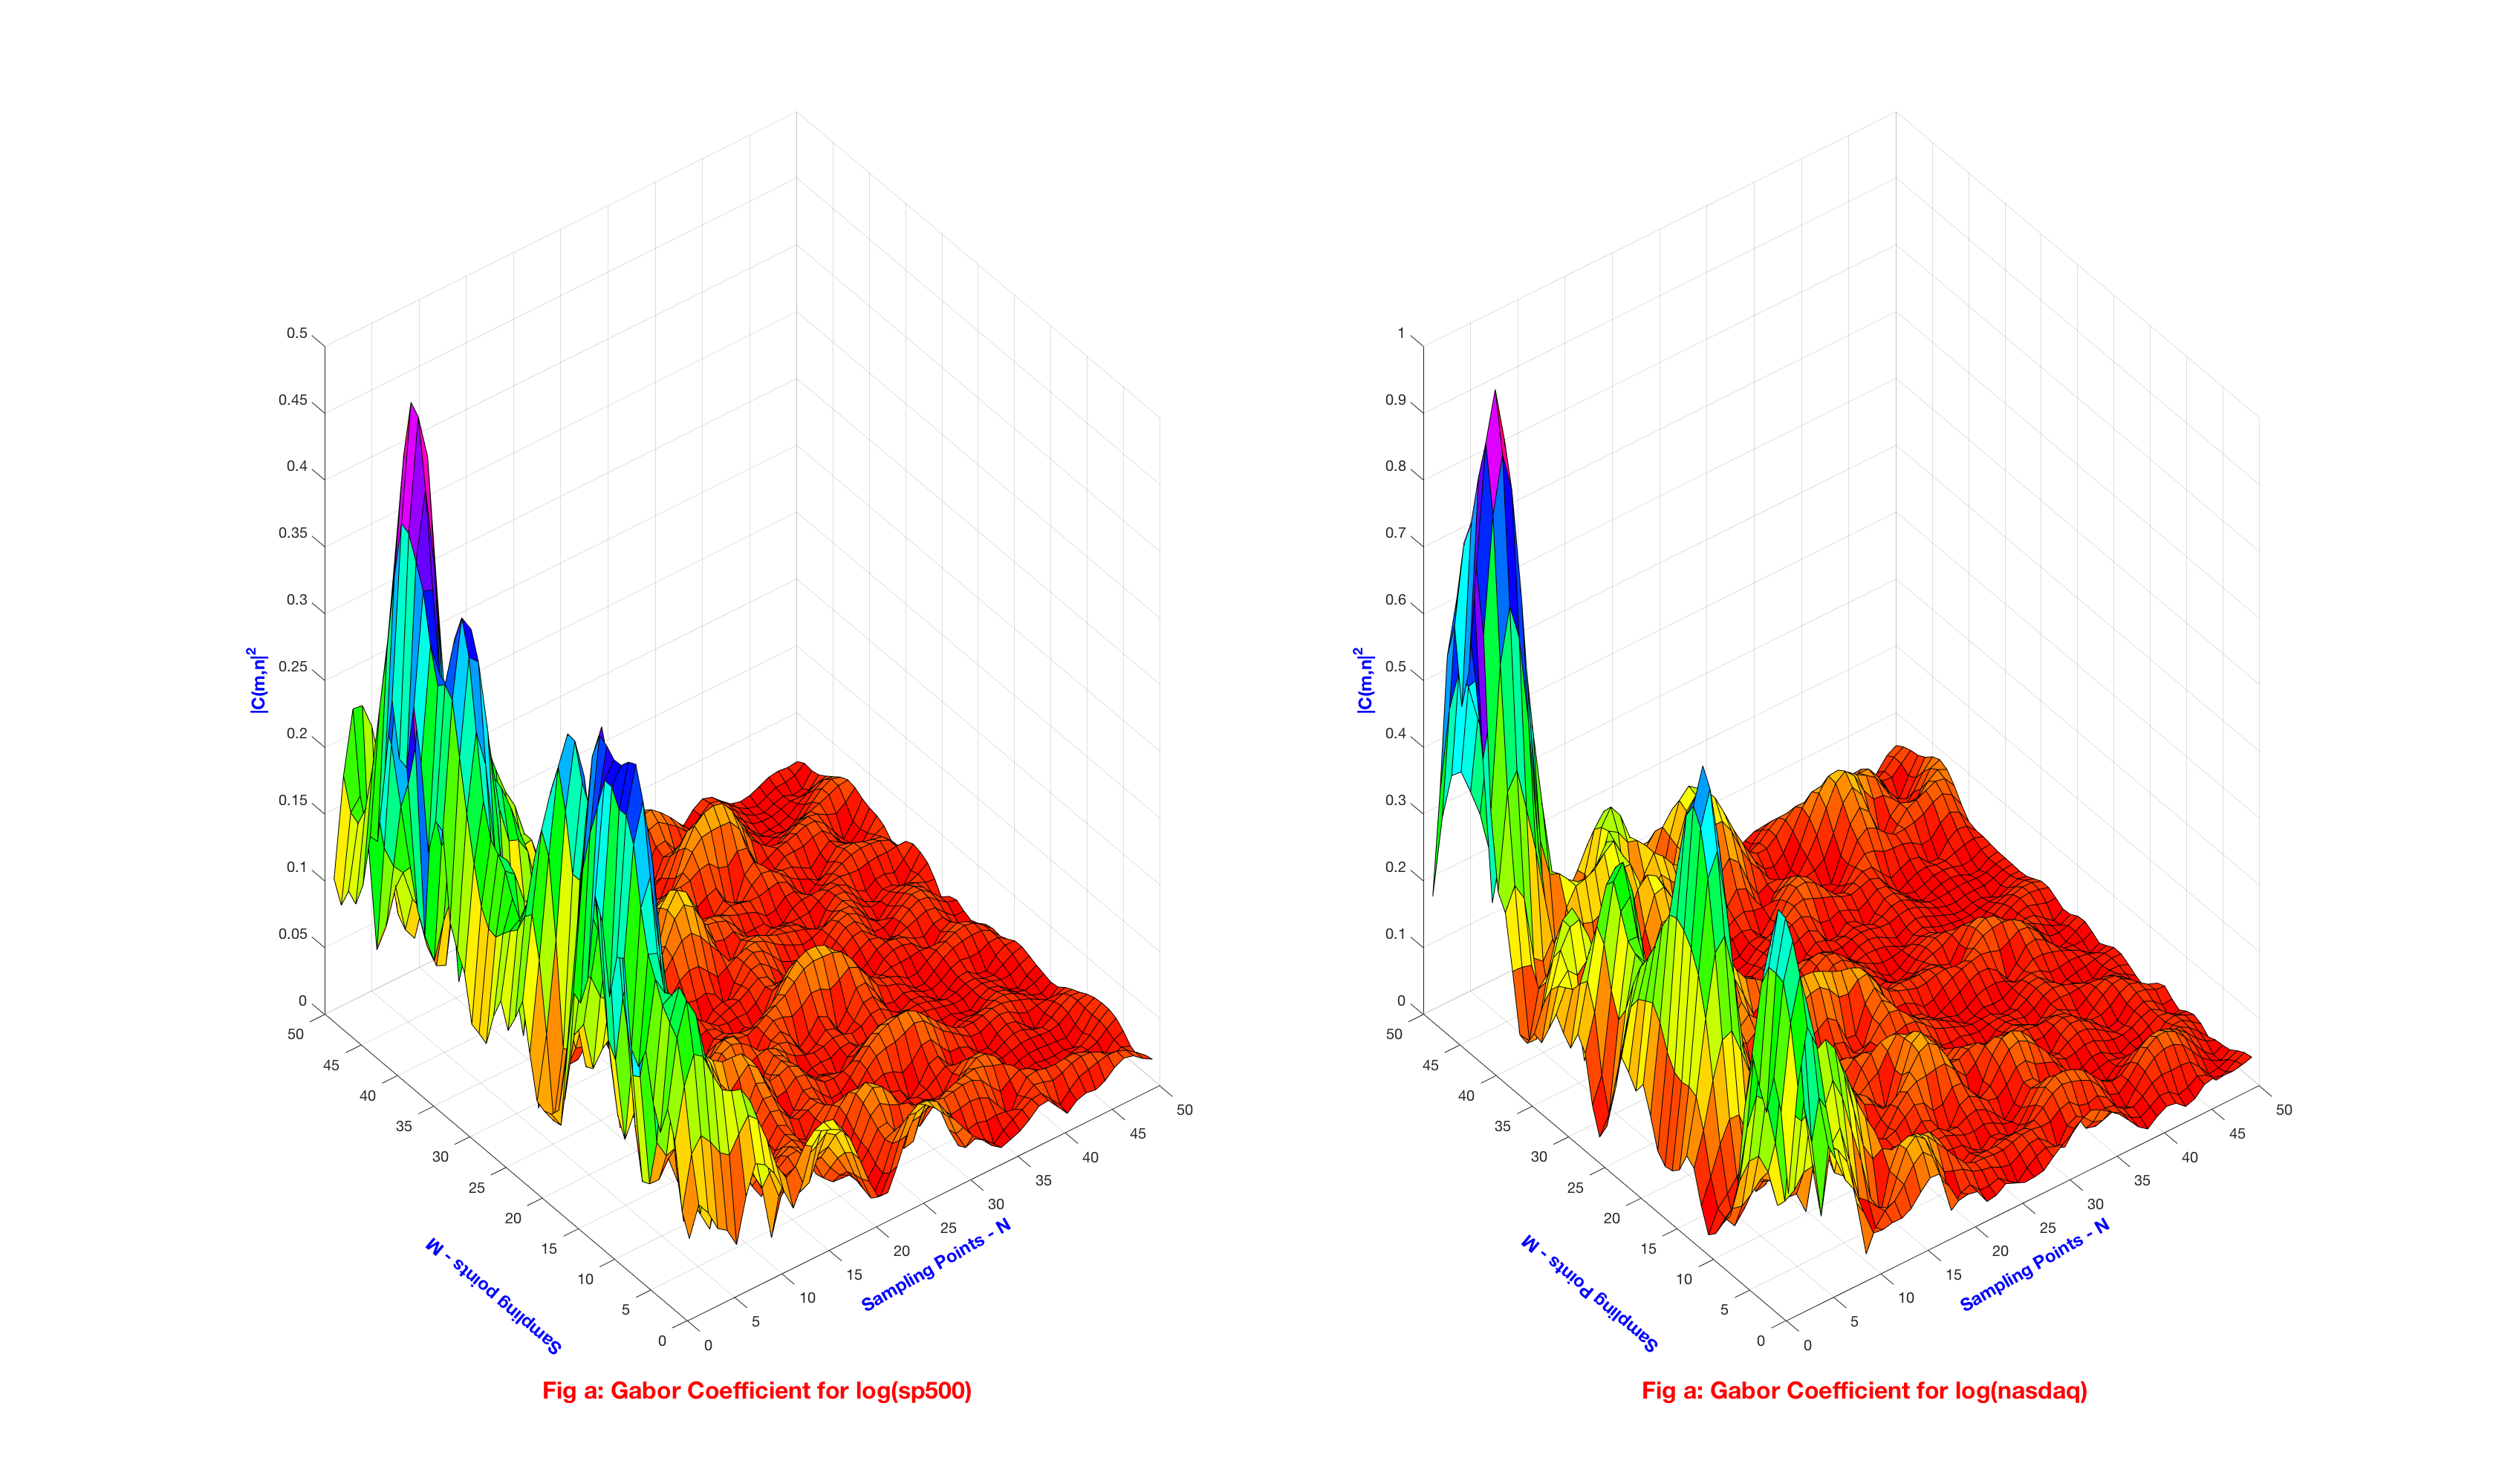
\includegraphics[scale=.15]{Images/GaborThreshold50}
\caption{Fig a is the time section of Gabor distribution of HP Filter cycles log(SP500) and Fig b is the time section of Gabor distribution of for HP Filter cycles log(NASDAQ). $\Delta M = 8; \Delta N = 4; m = 50; n = 100; \sigma = \sqrt{\frac{\Delta M L}{\Delta N 2\pi}}$. Threshold is calculated as $max(|c(m,n)|-min(|c(m,n)|))/2$. The program used to create the graph is mygaborfilt.m and it is attached in the appendix.}
\label{fig:GaborThreshold50}
\end{figure}

\begin{figure}[!ht]
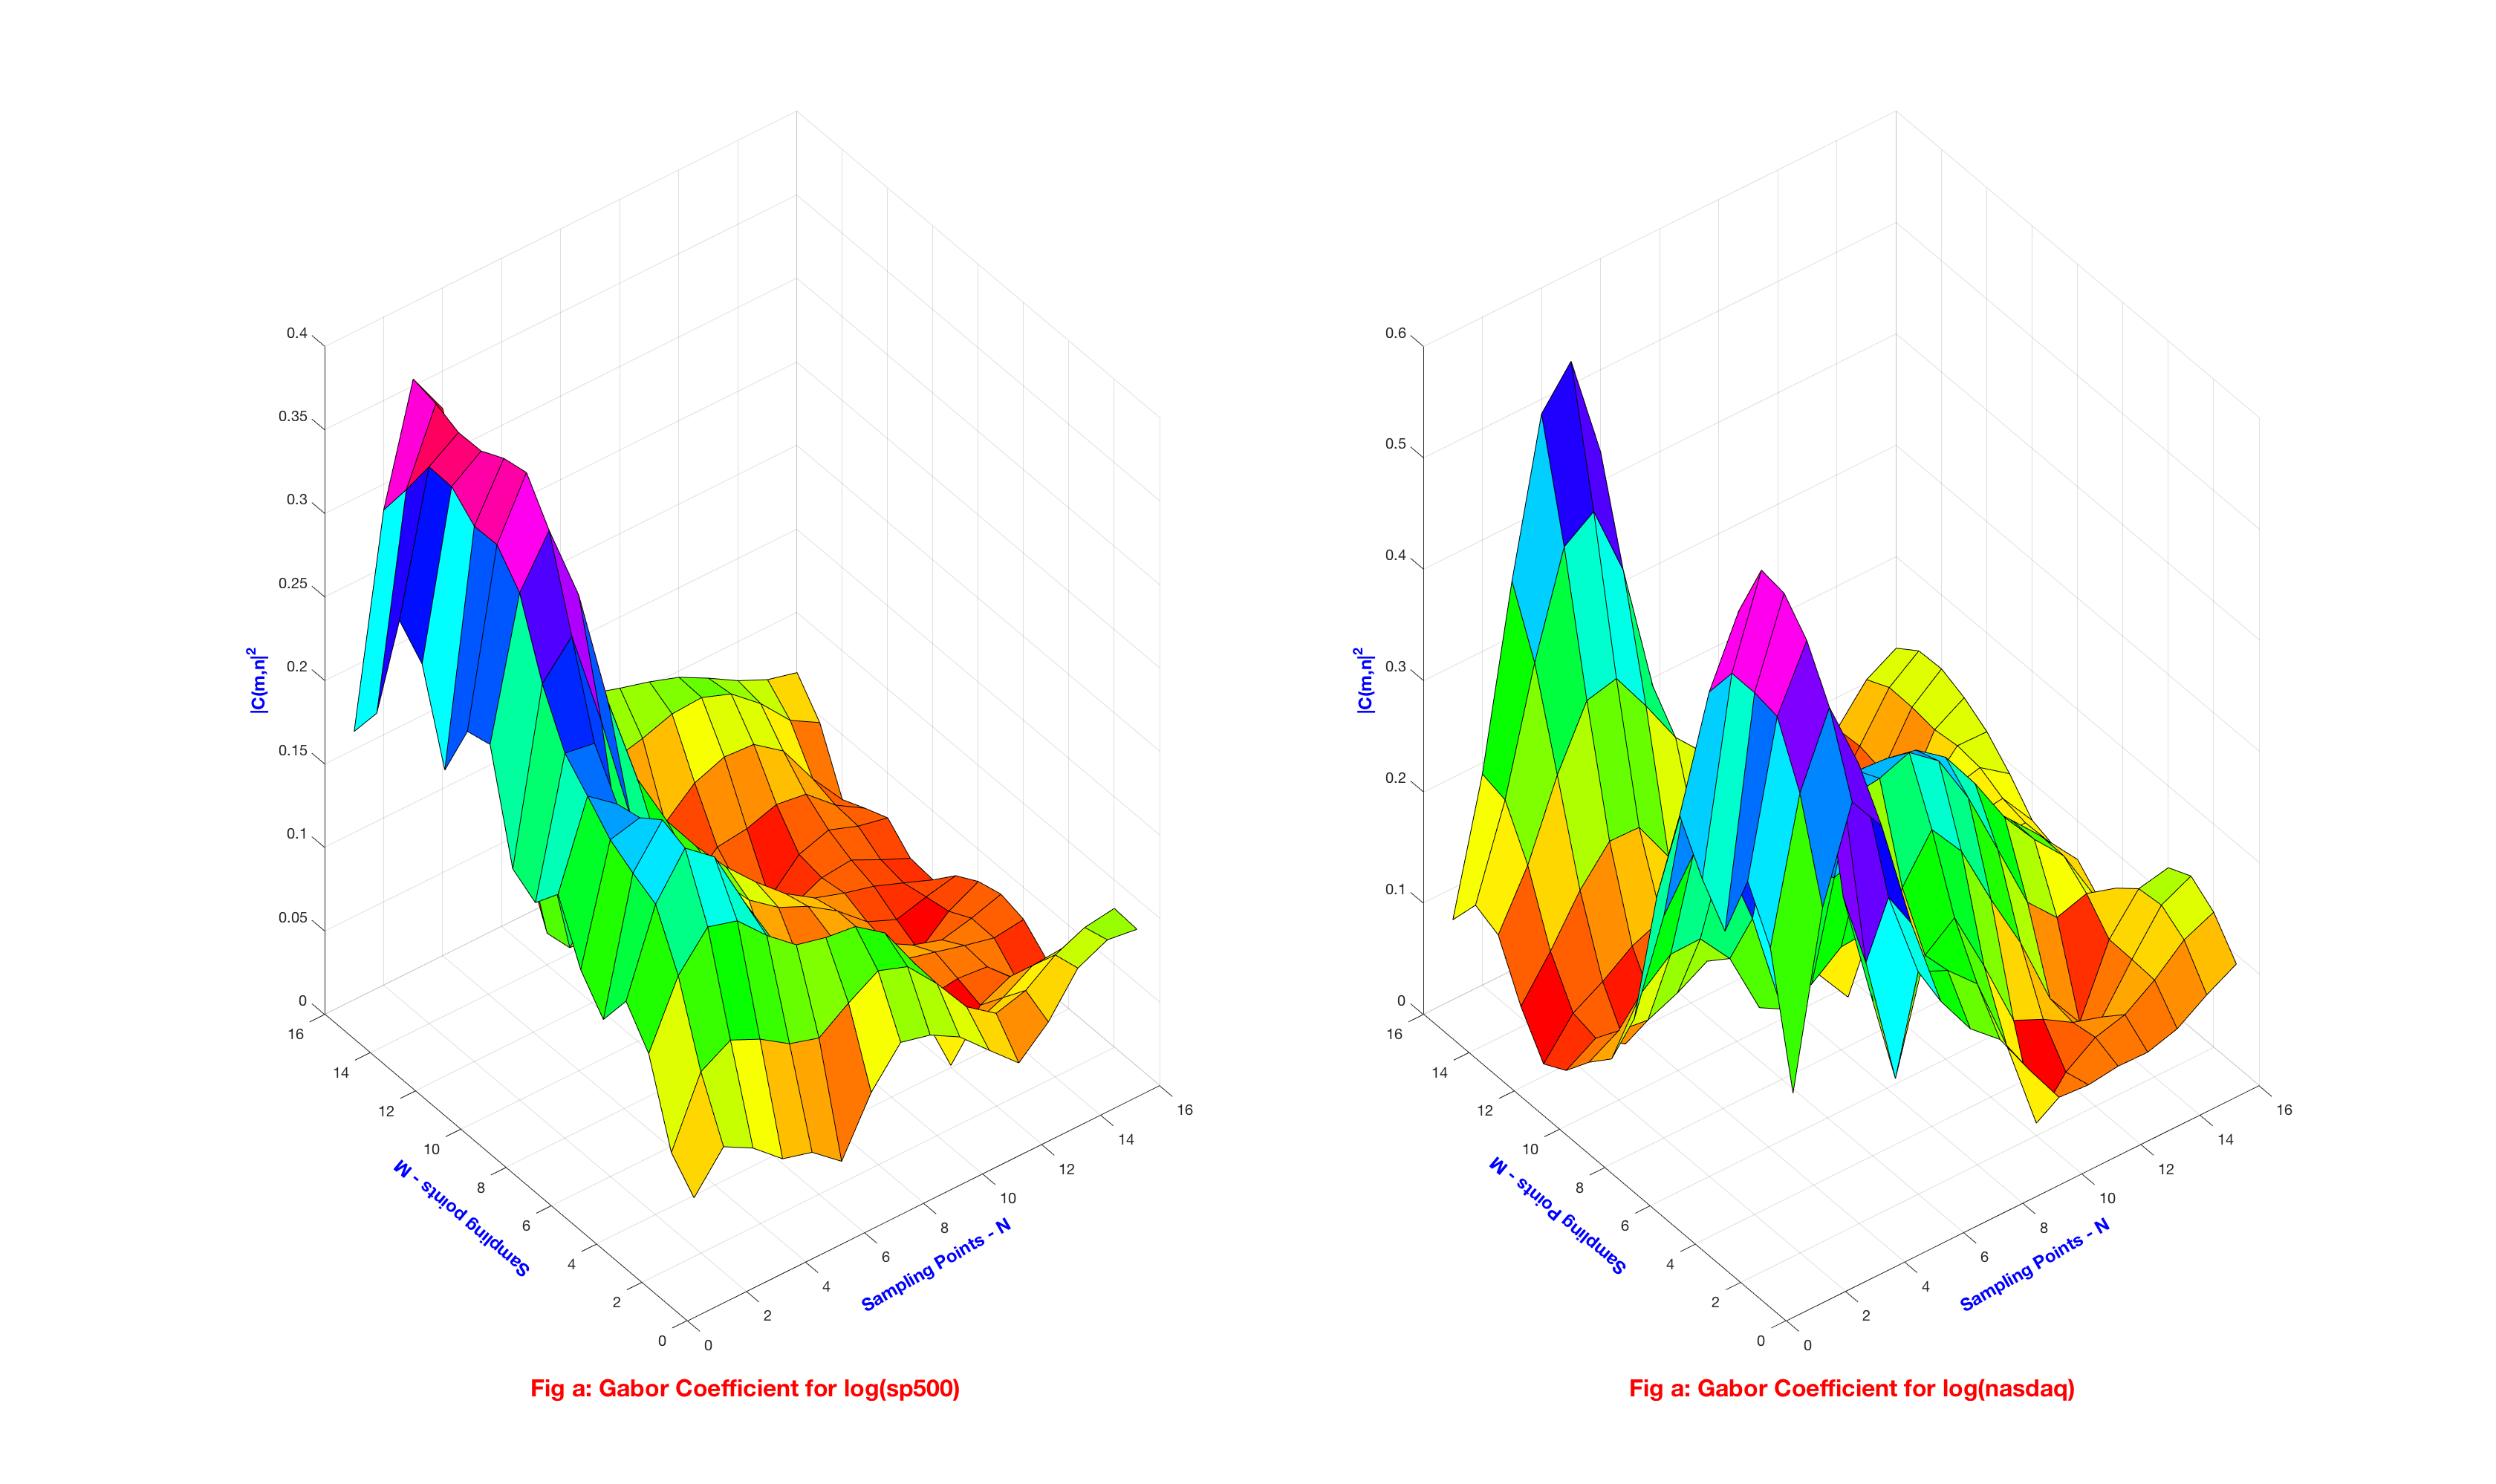
\includegraphics[scale=.15]{Images/GaborThreshold16}
\caption{Fig a is the time section of Gabor distribution of HP Filter cycles log(SP500) and Fig b is the time section of Gabor distribution of for HP Filter cycles log(NASDAQ). $\Delta M = 8; \Delta N = 4; m = 16; n = 32; \sigma = \sqrt{\frac{\Delta M L}{\Delta N 2\pi}}$. Threshold is calculated as $max(|c(m,n)|-min(|c(m,n)|))/2$. The program used to create the graph is mygabor.m and it is attached in the appendix.}
\label{fig:GaborThreshold16}
\end{figure}


\begin{comment}
Gabor co-efficient $C_{m,n}$ and synthesis function $f(t)$ are bi-orthogonal functional sets.  \\
\begin{equation}
C_{m,n} = \sum_{m,n\in Z} \psi_{m,n}^*(t) f(t)
\end{equation}
$\psi_{m,n}^*$ is the complex conjugate of $\psi_{m,n}$.\\
\\
\end{comment}
The GEFs could be a set of Gaussian functions modulated by simple harmonics. GEFs are generated in 1D by combining Gaussian and simple harmonic functions. The Gaussian function remained the same for both GEF and only the sinusoidal functions changed between the two GEFs. Note the change in the frequency between the GEFs. A set of GEFs can be created by varying ma and nb.\\
\begin{equation*}
\psi_{m,n}(t) =  e^{-\frac{(t-\mu-ma)^2}{2\sigma^2}} e^{j2\pi nbt}
\end{equation*}

If the GEF $\psi$ and its Fourier transform (frequency representation) $\Psi$ are localized at the origin then $\psi_{m,n}$ is localized at (ma,nb) in the joint time-frequency domain. Each GEF occupies a region in time-frequency plane and associated $C_{m,n}$ represents a quantum of information.\\

Let $\psi(t)$ be a GEF. The GEF in the frequency domain is given by the Fourier transform \\
\begin{equation*}
\Psi(f) = \int_{-\infty}^{\infty}\psi(t) e^{-j2\pi ft}\, dt \\
\end{equation*}

These functions have a special property that relates to Heisenberg's uncertainty principle. The product of the standard deviation in time $\Delta t$ and variance in frequency $\Delta f$ is always greater than or equal to a certain quantity.
\begin{equation}
\Delta f \Delta t \geq \frac{1}{4\pi}
\end{equation}
The time standard deviation or effective duration and frequency variance or effective frequency width can be calculated by the root mean square (RMS) deviation of the signal from the mean. The effective duration ($\Delta t$) and effective frequency width ($\Delta f$) are given by
\begin{equation*}
\Delta t = \sqrt{\frac{\int_{-\infty}^{\infty}{\psi(t)(\mu_t - t)^2\psi ^*(t)dt}}{\int_{-\infty}^{\infty}{\psi(t)\psi ^*(t)dt}}} ;
\Delta f = \sqrt{\frac{\int_{-\infty}^{\infty}{\Psi(f)(\mu_f - f)^2\Psi ^*(f)df}}{\int_{-\infty}^{\infty}{\Psi(f)\Psi ^*(f)df}}}
\end{equation*}

where $\mu_t$ and $\mu_f$ are mean time and mean frequency and they are given by
\begin{equation*}
\mu_t = \frac{\int_{-\infty}^{\infty}{\psi(t)t\psi ^*(t)}}{\int_{-\infty}^{\infty}{\psi(t)\psi ^*(t)}} ;
\mu_f = \frac{\int_{-\infty}^{\infty}{\Psi(f)f\Psi ^*(f)}}{\int_{-\infty}^{\infty}{\Psi(f)\Psi ^*(f)}}
\end{equation*}

\subsection{Mask Operator}
In general, random noise tends to spread evenly in the joint time-frequency domain, while the signal itself concentrates in a relatively small range. Consequently, by a joint time-frequency representation, the signal-to-noise ratio could be substantially improved. Once the interesting signal has been identified, we can apply a mask operator to eliminate the background noise. Typical procedure of the time-variant filter is first to take the Gabor transform and then apply the mask operator to eliminate the background noise to obtain noiseless Gabor coefficients. 

\begin{figure}[!ht]
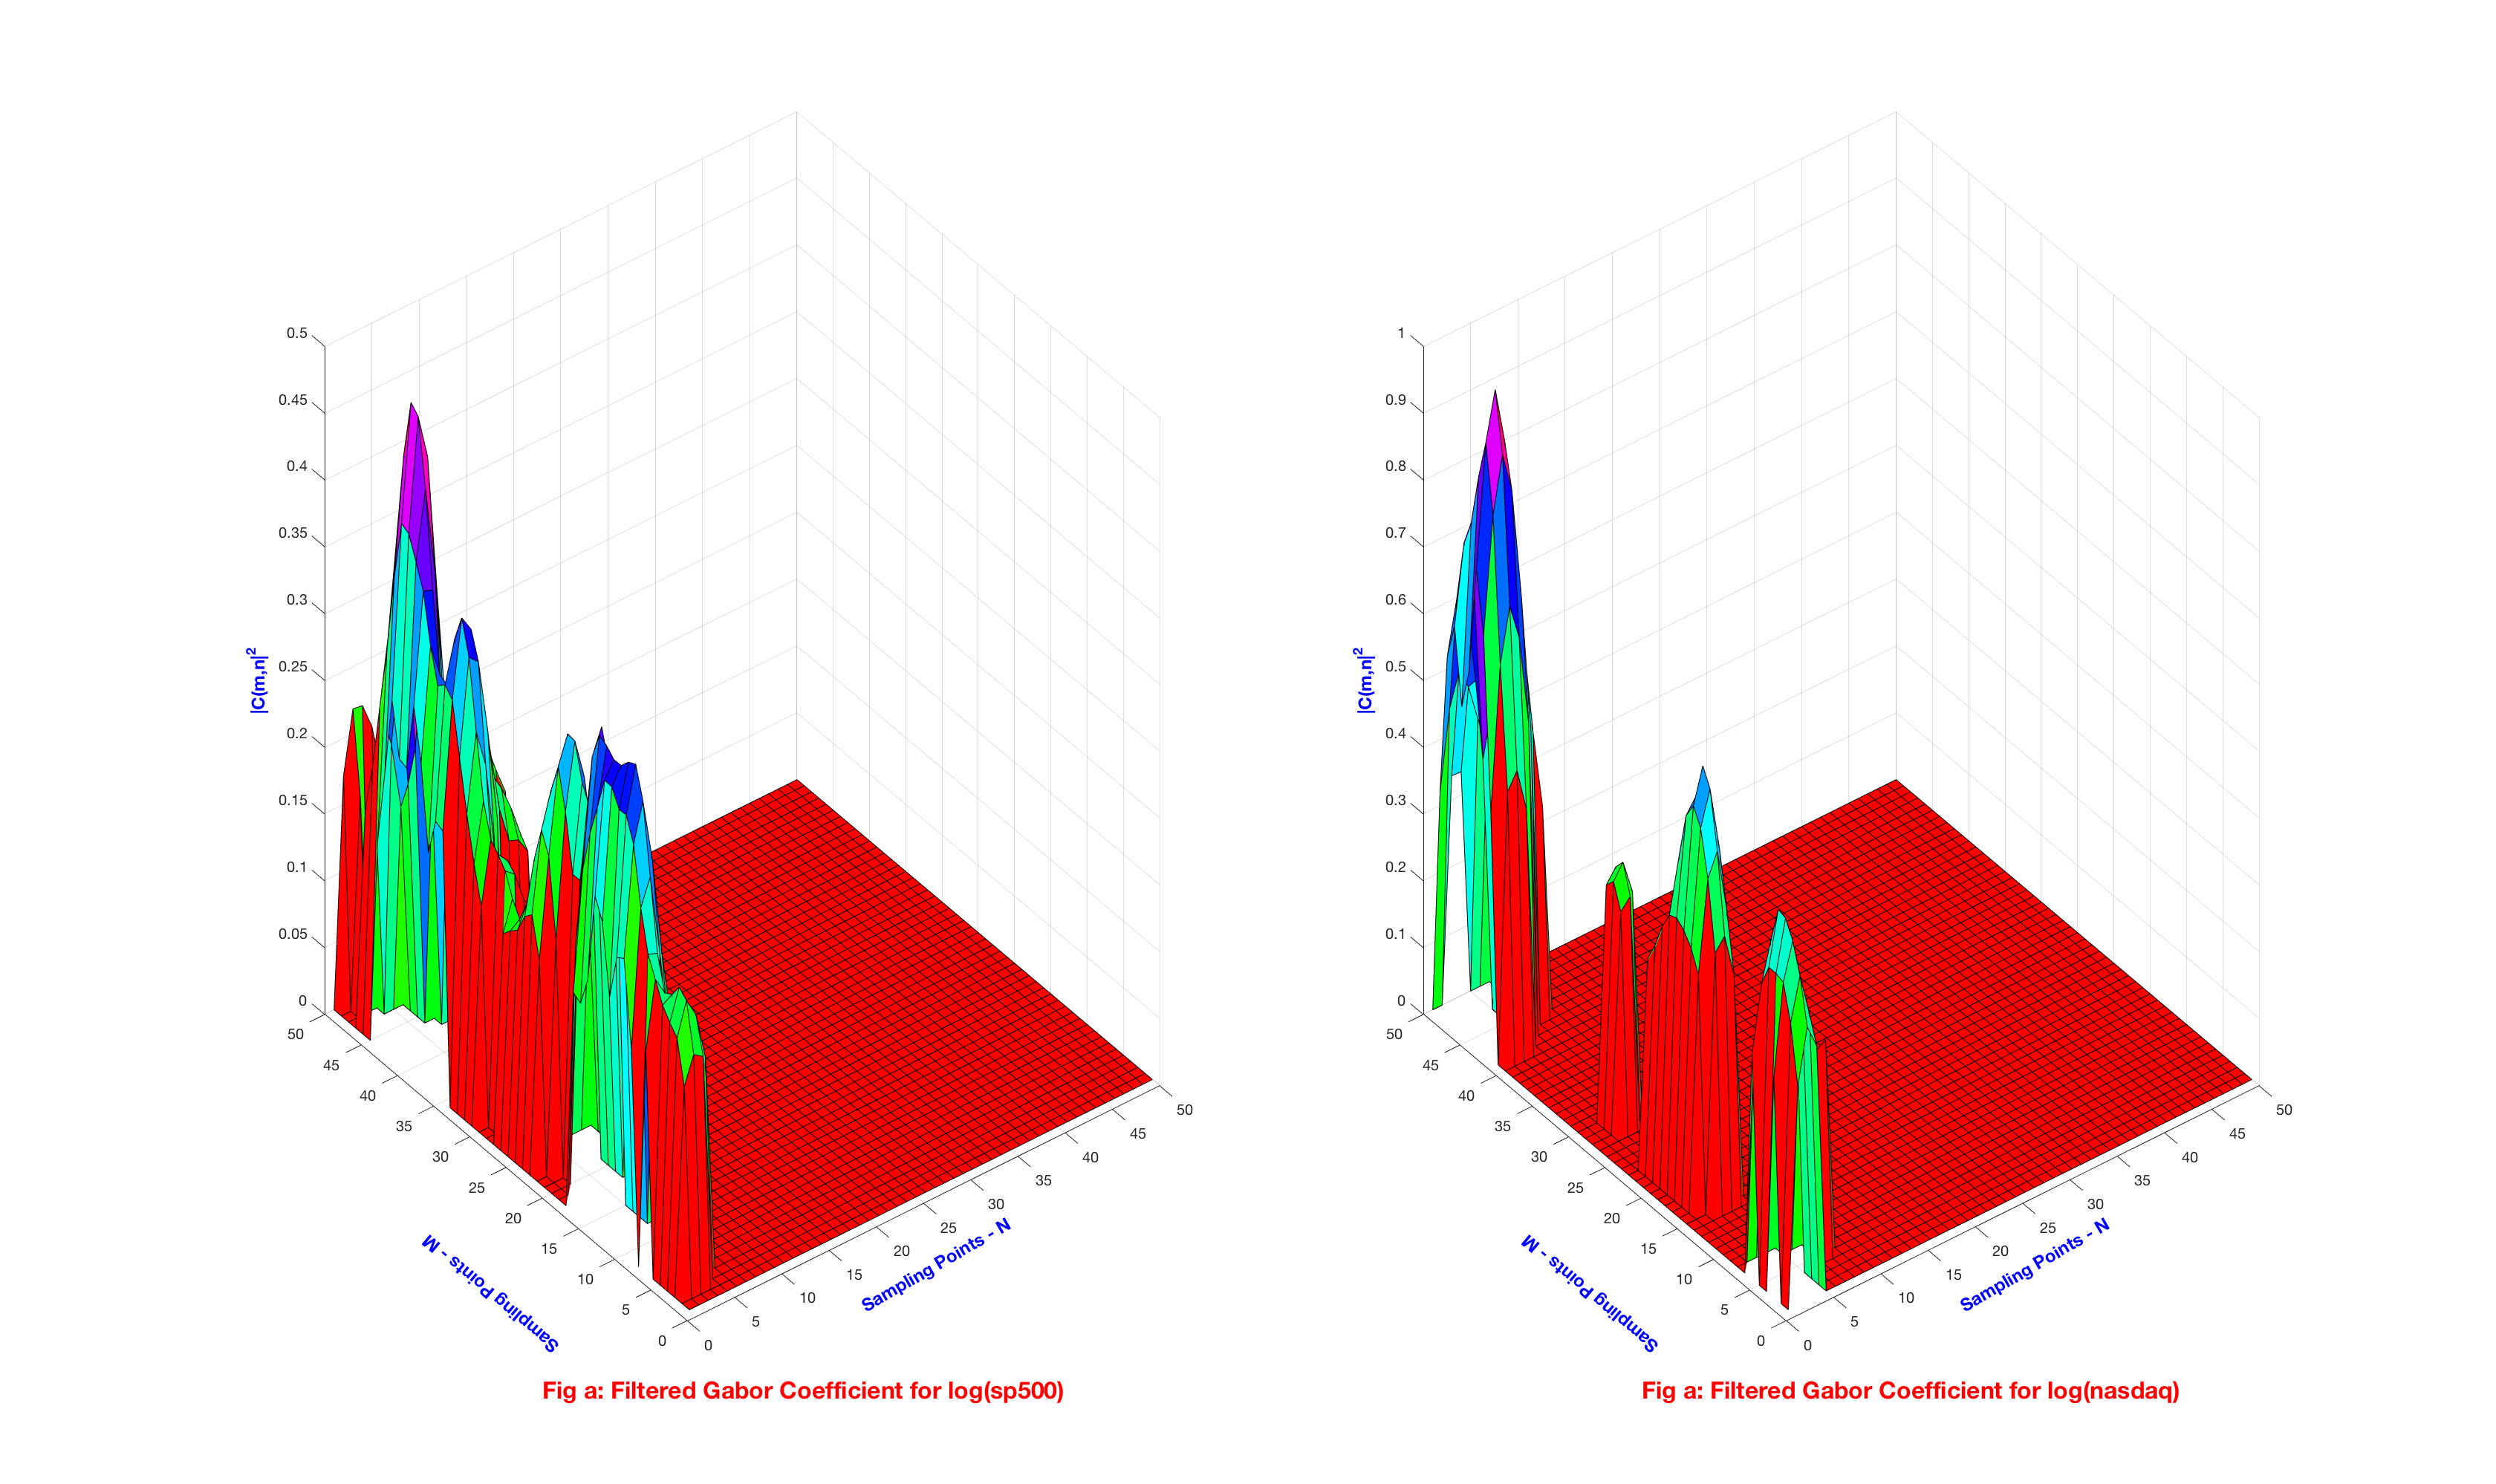
\includegraphics[scale=.15]{Images/GaborMasked50}
\caption{Fig a is the Filtered Gabor Coefficient for HP Filter cycles log(SP500) and Fig b is the Filtered Gabor Coefficient for HP Filter cycles log(NASDAQ).$\Delta M = 8; \Delta N = 4; m = 50; n = 100; \sigma = \sqrt{\frac{\Delta M L}{\Delta N 2\pi}}$. The mask operator is created based on the threshold of a peak distribution. The program used to create the graph is myfiltgabor.m and it is attached in the appendix.}
\label{fig:GaborMasked50}
\end{figure}

\begin{figure}[!ht]
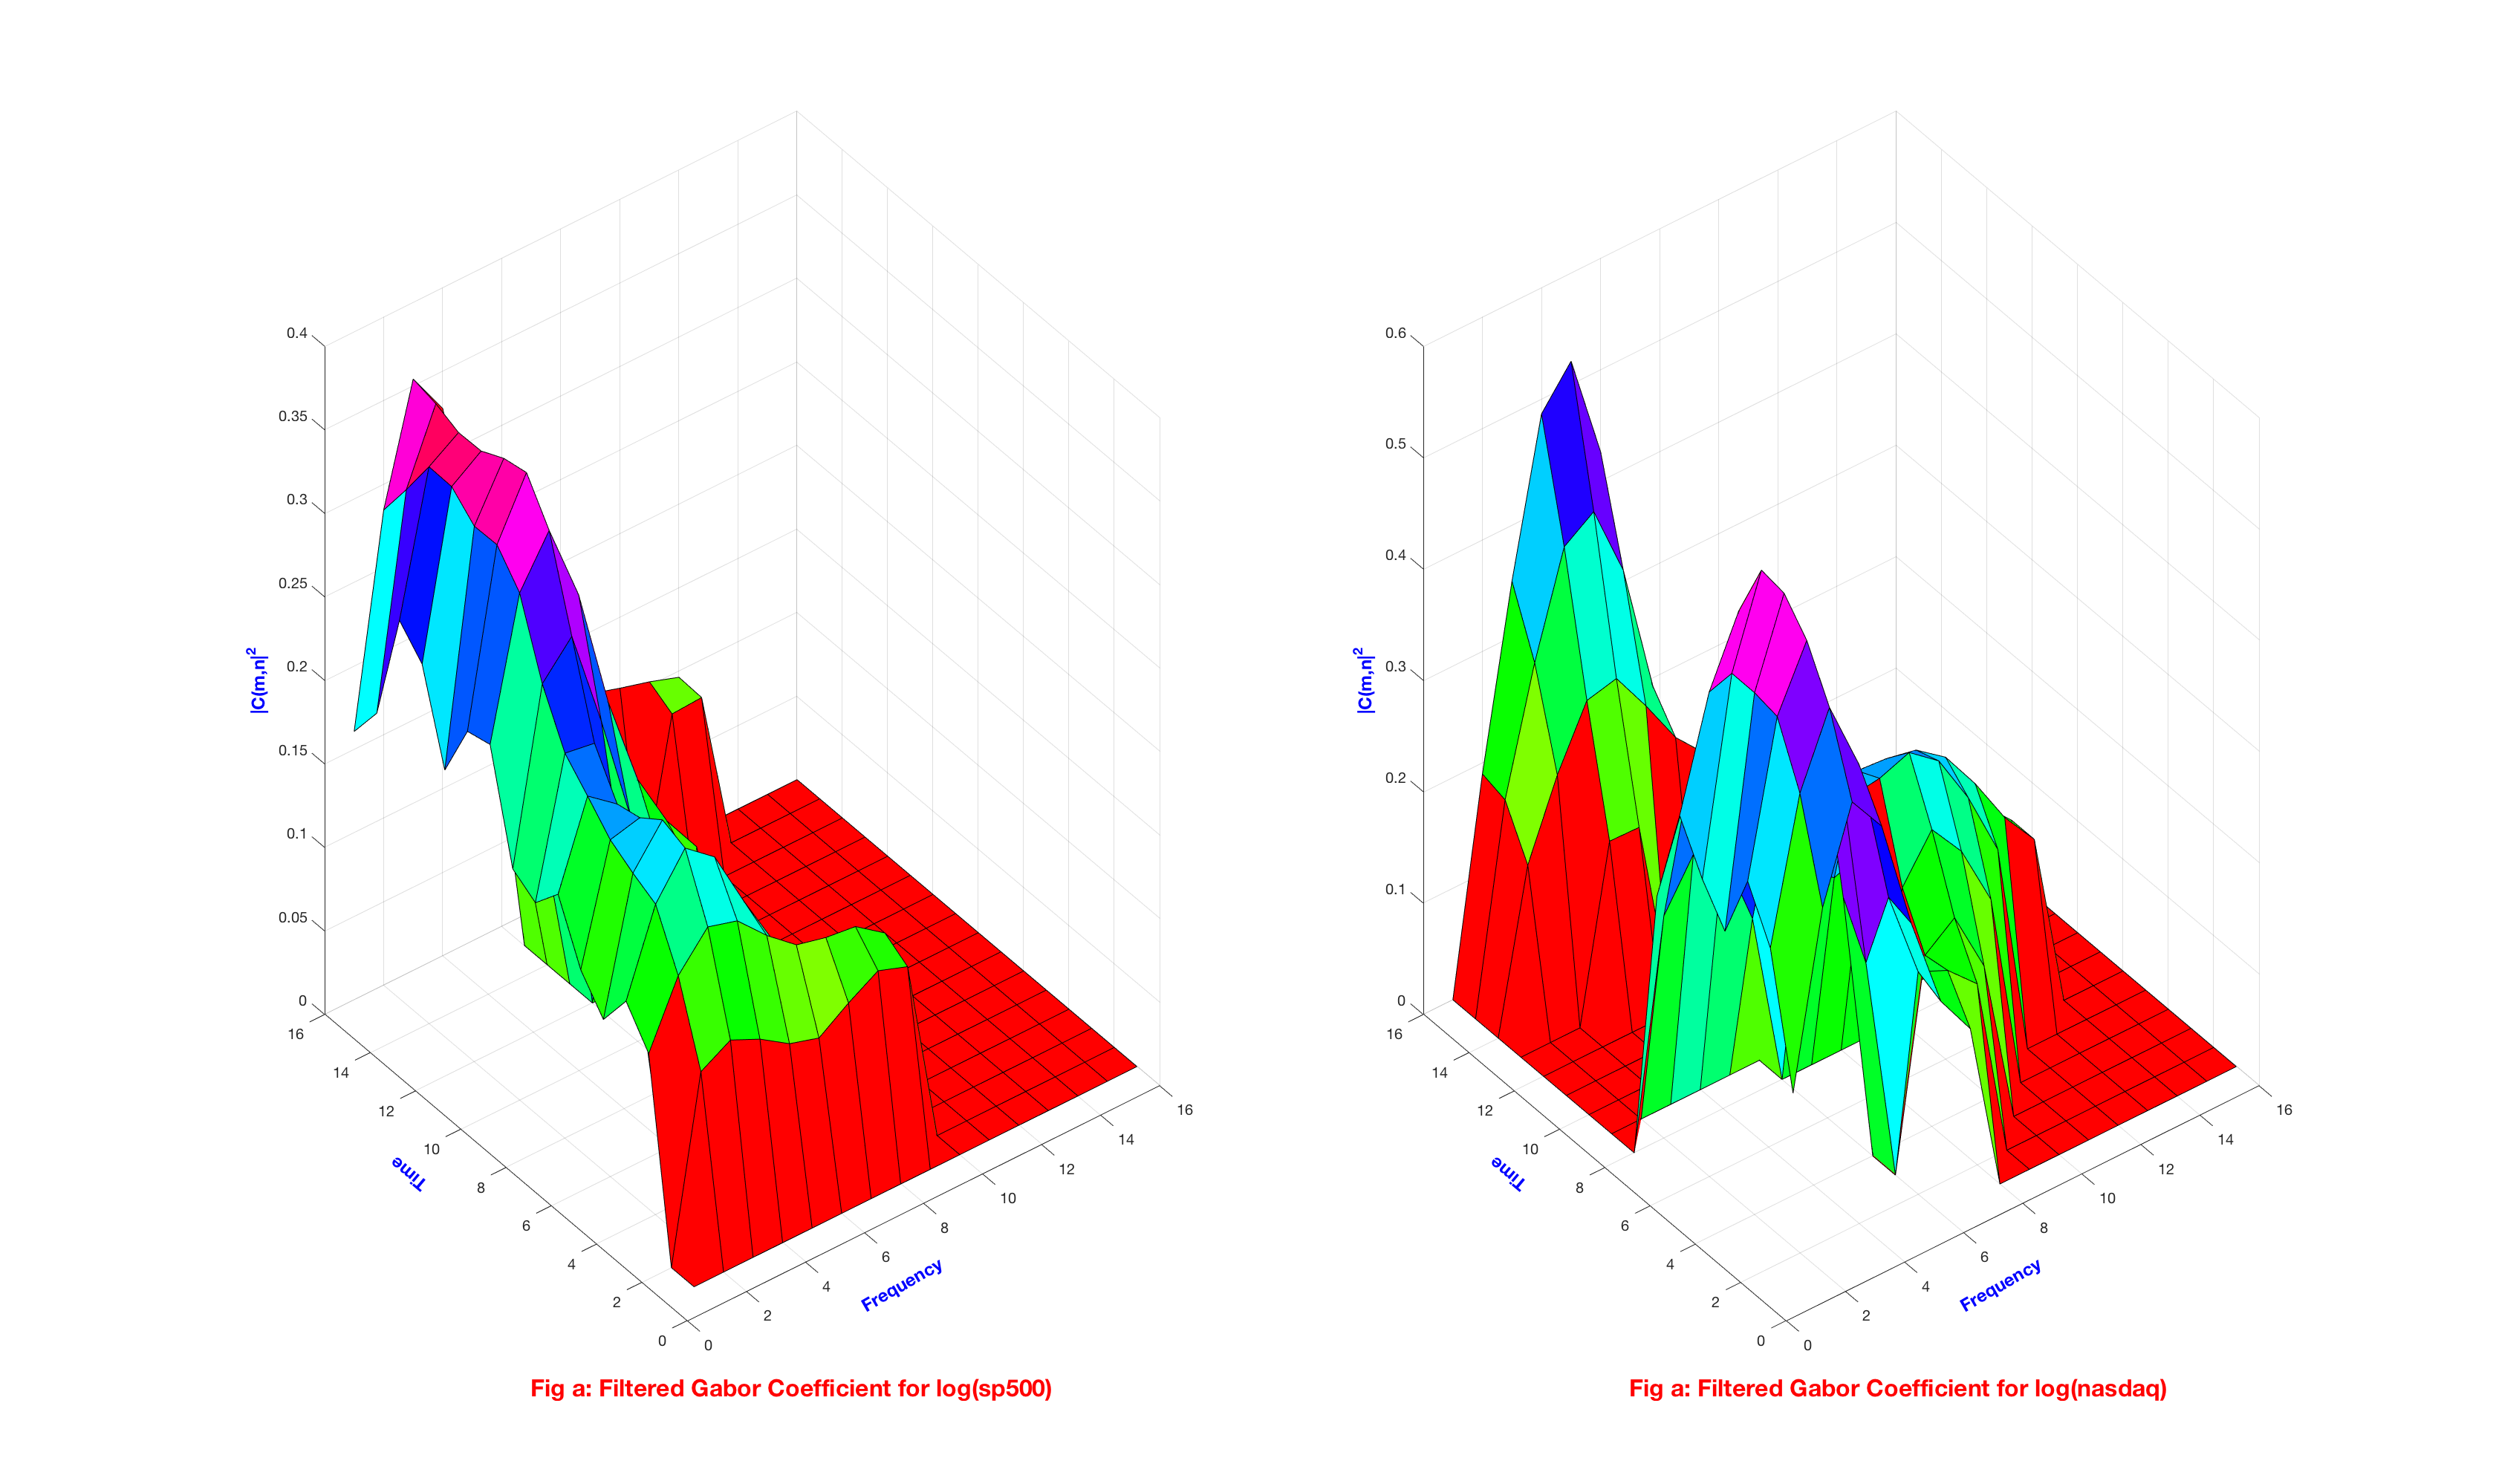
\includegraphics[scale=.15]{Images/GaborMasked16}
\caption{Fig a is the Filtered Gabor Coefficient for HP Filter cycles log(SP500) and Fig b is the Filtered Gabor Coefficient for HP Filter cycles log(NASDAQ).$\Delta M = 8; \Delta N = 4; m = 16 ;n = 32 ; \sigma = \sqrt{\frac{\Delta M L}{\Delta N 2\pi}}$. The mask operator is created based on the threshold of a peak distribution. The program used to create the graph is myfiltgabor.m and it is attached in the appendix.}
\label{fig:GaborMasked16}
\end{figure}

\begin{figure}[!ht]
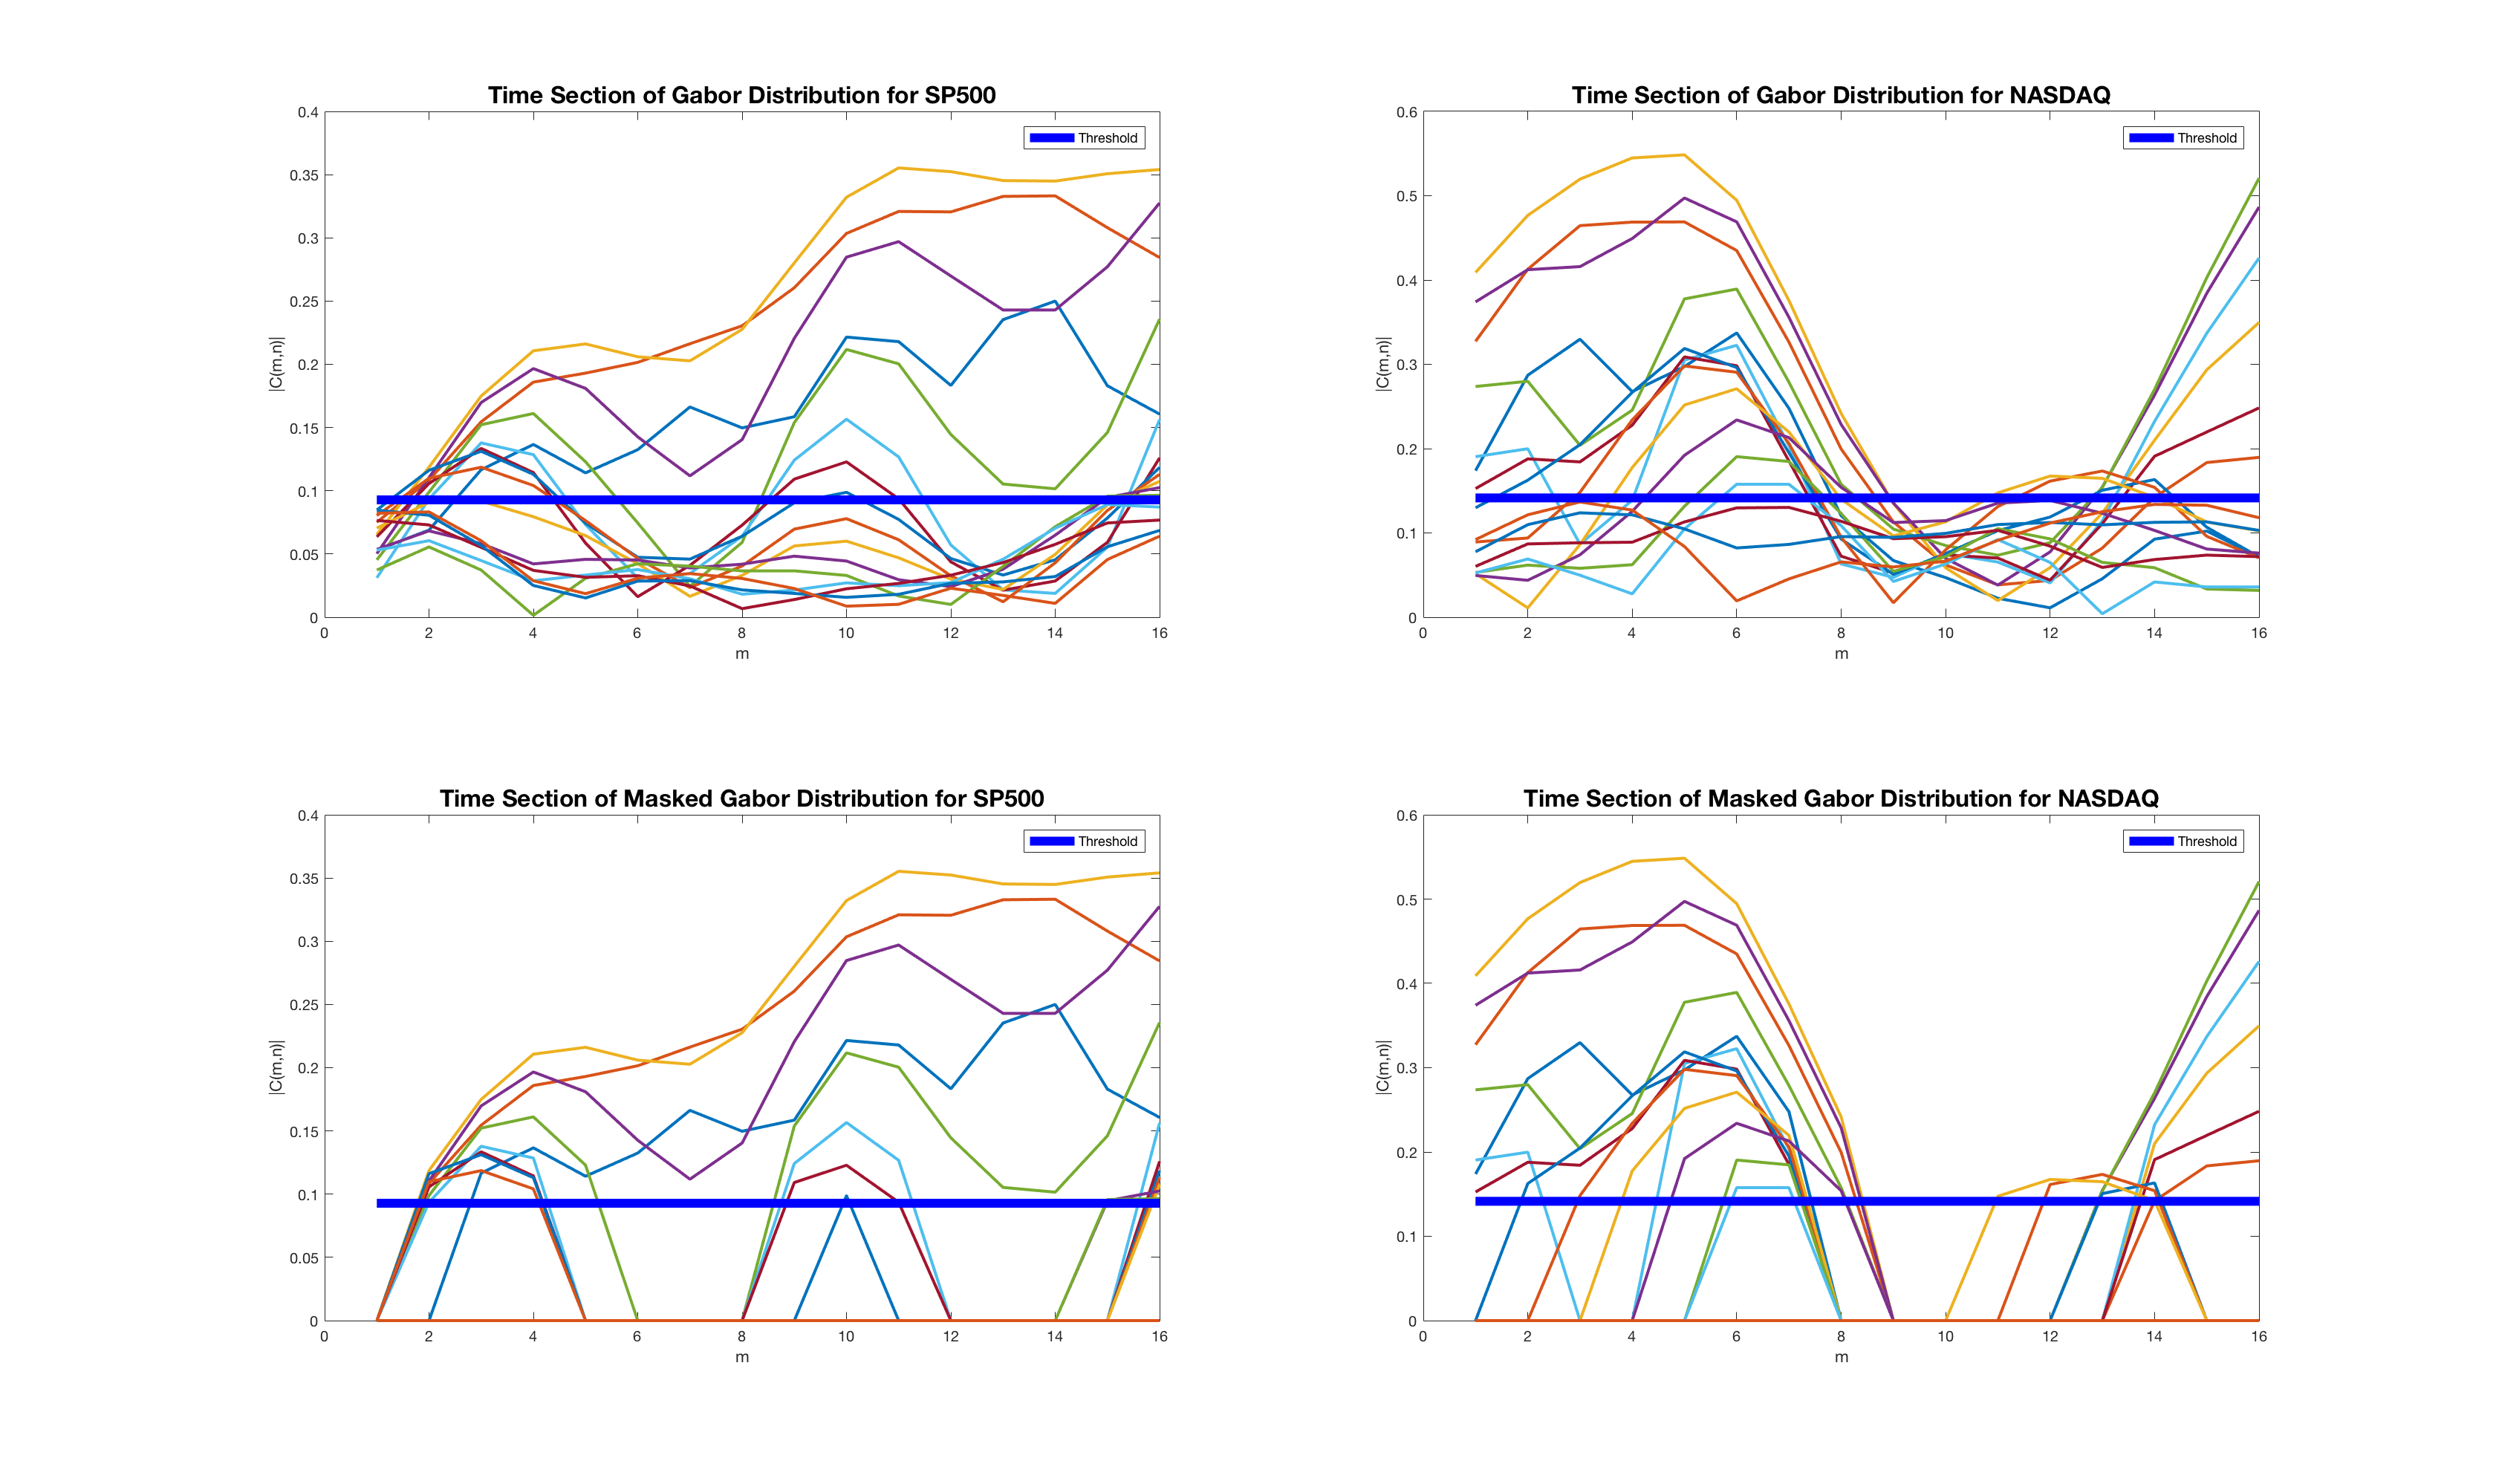
\includegraphics[scale=.15]{Images/GaborPST16}
\caption{Fig a is the time section of Gabor distribution of HP Filter cycles log(SP500) and Fig b is the time section of Gabor distribution of for HP Filter cycles log(NASDAQ). $\Delta M = 8; \Delta N = 4; m = 16; n = 32; \sigma = \sqrt{\frac{\Delta M L}{\Delta N 2\pi}}$. Threshold is calculated as $max(|c(m,n)|-min(|c(m,n)|))/2$. Mask operator used to eliminate values below threshold. The program used to create the graph is mygaborfilt.m and it is attached in the appendix.}
\label{fig:GaborPST16}
\end{figure}


\begin{figure}[!ht]
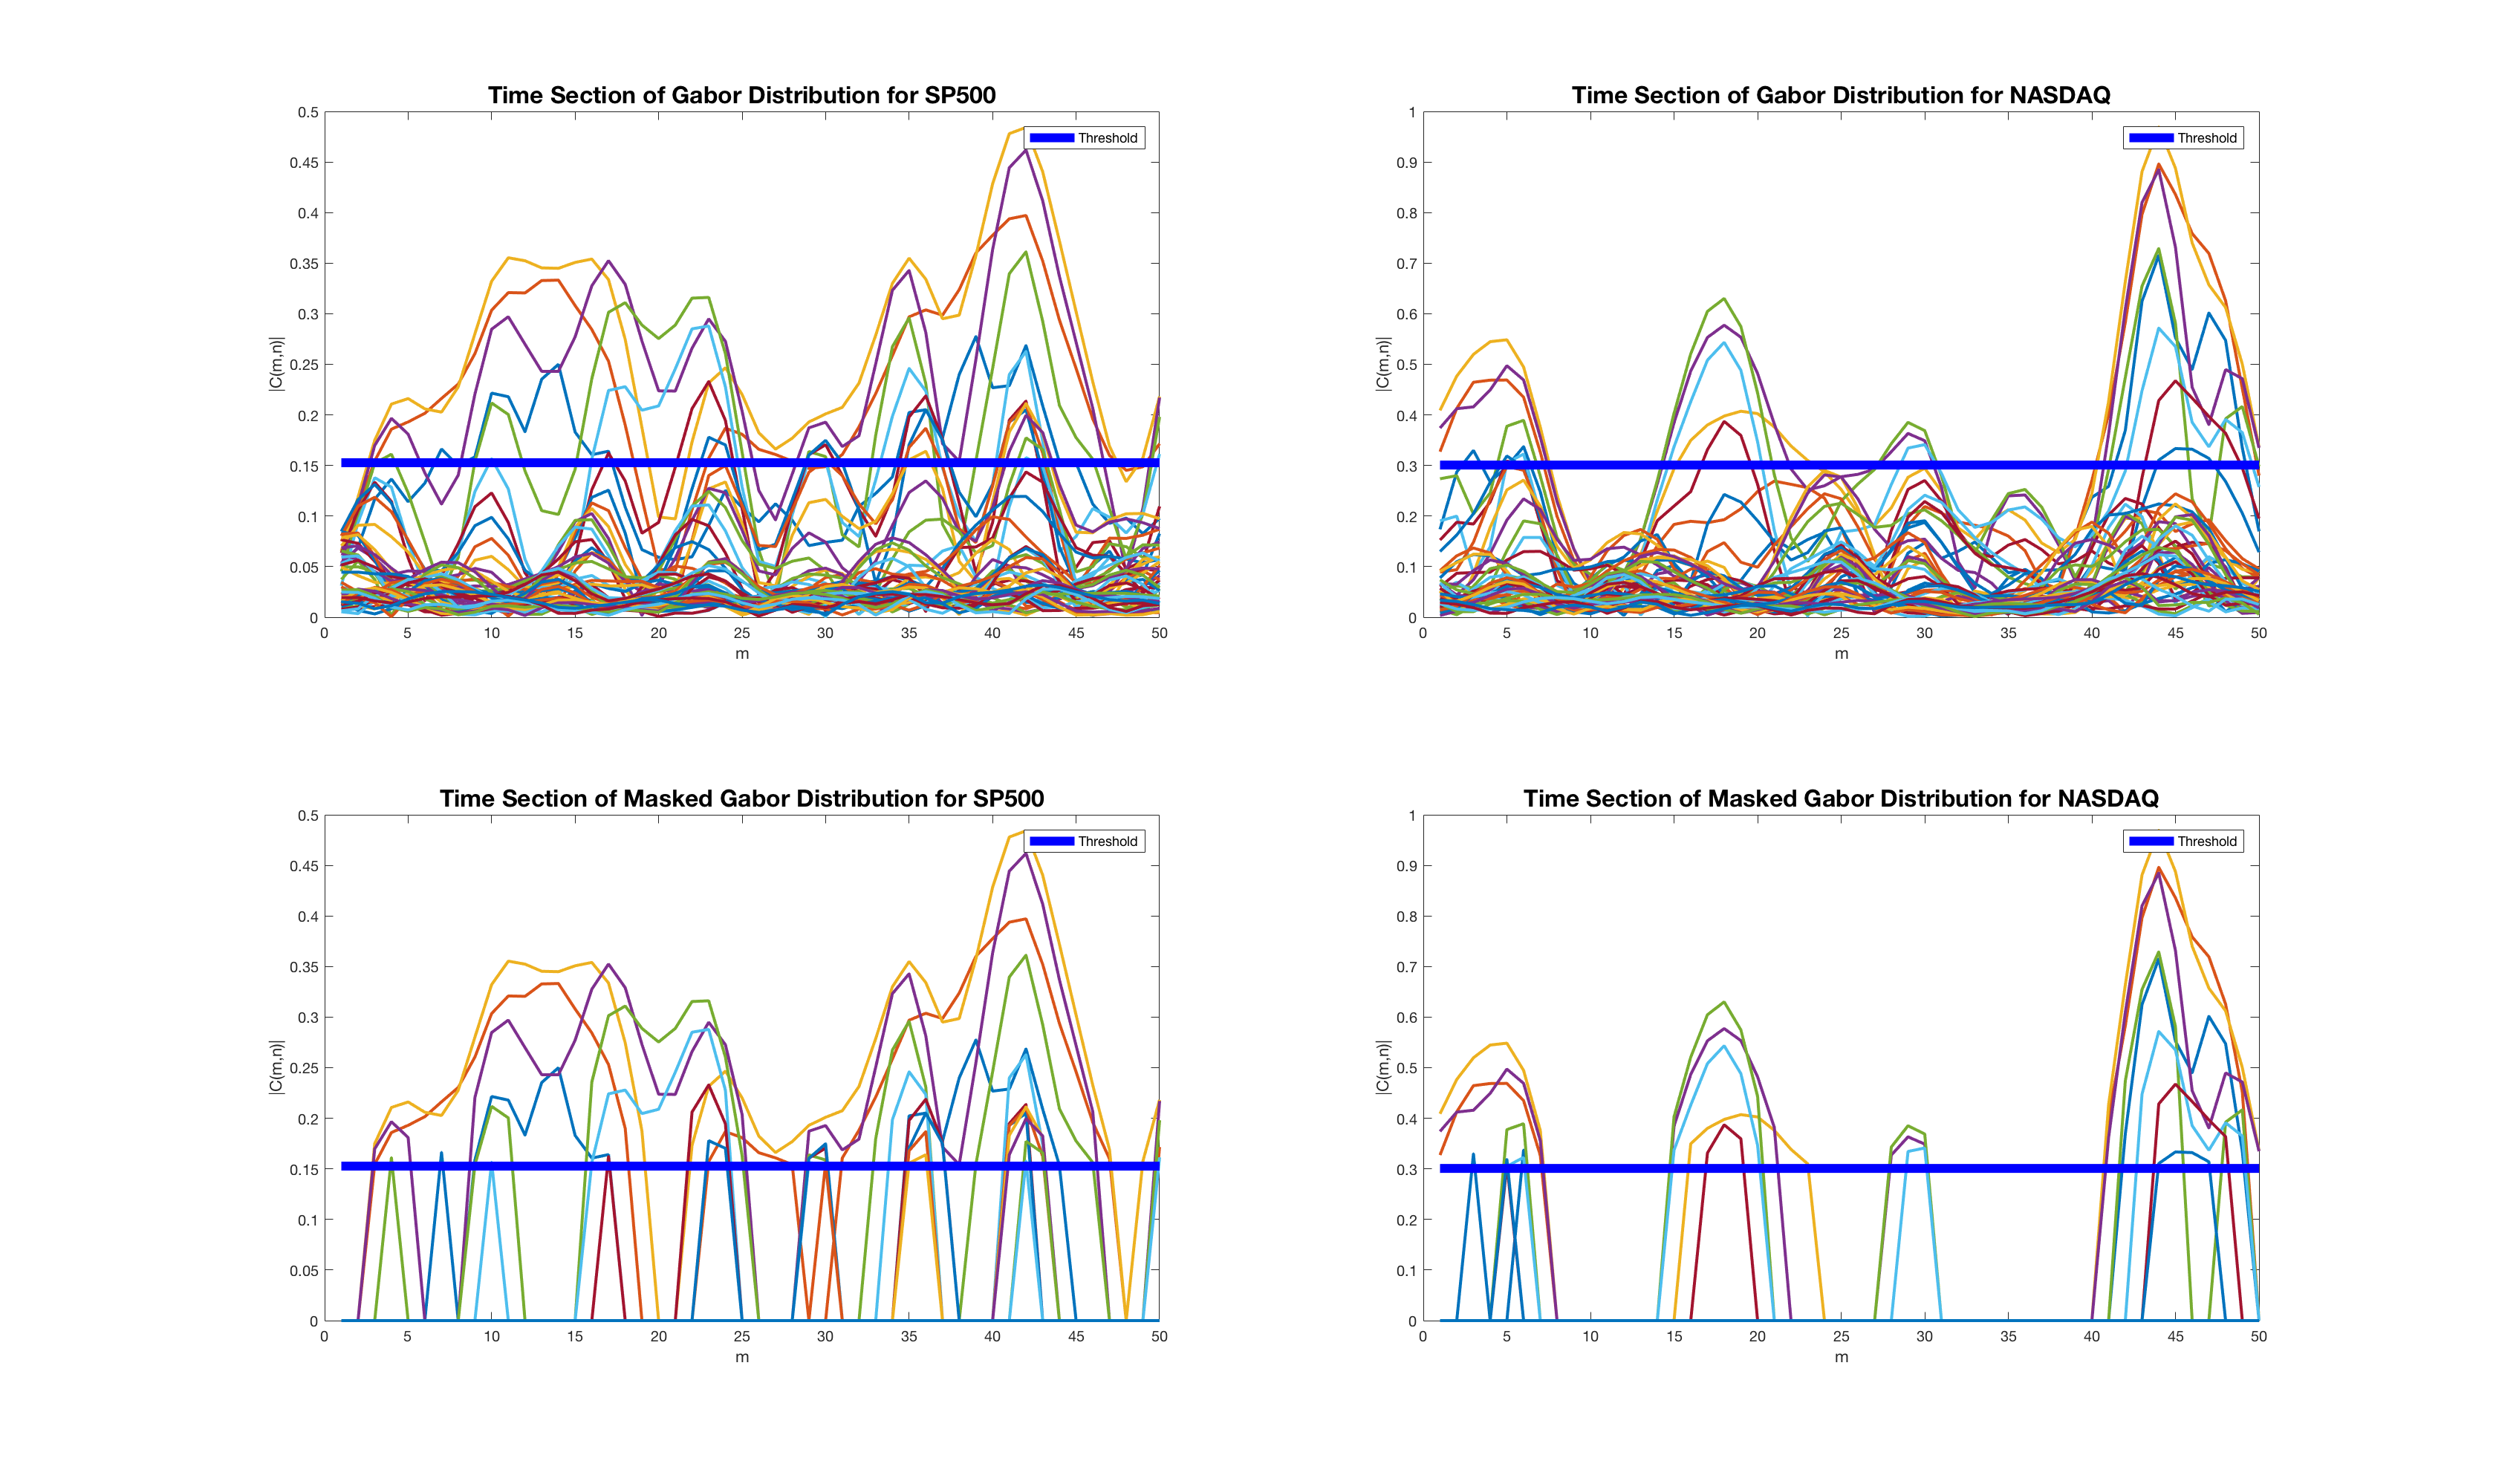
\includegraphics[scale=.15]{Images/GaborPST50}
\caption{Fig a is the time section of Gabor distribution of HP Filter cycles log(SP500) and Fig b is the time section of Gabor distribution of for HP Filter cycles log(NASDAQ). $\Delta M = 8; \Delta N = 4; m = 50; n = 100; \sigma = \sqrt{\frac{\Delta M L}{\Delta N 2\pi}}$. Threshold is calculated as $max(|c(m,n)|-min(|c(m,n)|))/2$. Mask operator used to eliminate values below threshold. The program used to create the graph is mygaborfilt.m and it is attached in the appendix.}
\label{fig:GaborPST50}
\end{figure}



\begin{equation*}
\Delta t\Delta f = \sqrt{\frac{\int_{-\infty}^{\infty}{\psi(t)(\mu_t - t)^2\psi ^*(t)dt}}{\int_{-\infty}^{\infty}{\psi(t)\psi ^*(t)dt}} \frac{\int_{-\infty}^{\infty}{\Psi(f)(\mu_f - f)^2\Psi ^*(f)df}}{\int_{-\infty}^{\infty}{\Psi(f)\Psi ^*(f)df}}} \geq \frac{1}{4\pi}
\end{equation*}


There are three possibilities for the above equation given below in table ~\ref{table:sampling} .

\begin{table}[h!]
\centering
\begin{tabular}{|c|c|c|ccc|}
  \hline
  % after \\: \hline or \cline{col1-col2} \cline{col3-col4} ...
  \textbf{$\Delta t$  $\Delta f$} & \textbf Sampling & Remarks \\
  \hline
  = $\frac{1}{4\pi}$ & Critical   & Special functions called GEF \\
  \hline
   $>$ $\frac{1}{4\pi}$ & Over   & -- \\
  \hline
  $<$ $\frac{1}{4\pi}$ & Under   & This case is not possible \\
  \hline
\end{tabular}
\caption{Possible values for $\Delta$t $\Delta$f and special case for Gabor function}
\label{table:sampling}
\end{table}

Analogous to 1D uncertainty principle, there are two 2D uncertainty principles constraining the effective width ($\Delta x$) and the effective length ($\Delta y$) of a signal $f(x,y)$ and the effective width ($\Delta u$) and the effective length ($\Delta v$) of its 2D Fourier transform $F(u,v)$. 2D Gabor transformation has wide application in image processing domain and the 2D analysis is out of scope for this project.  


\begin{equation*}
\Delta x\Delta u = \sqrt{\frac{\int_{-\infty}^{\infty}{\psi(x,y)(\mu_x - x)^2\psi ^*(x,y)dxdy}}{\int_{-\infty}^{\infty}{\psi(x,y)\psi ^*(x,y)dxdy}} \frac{\int_{-\infty}^{\infty}{\Psi(u,v)(\mu_u - u)^2\Psi ^*(u,v)dudv}}{\int_{-\infty}^{\infty}{\Psi(u,v)\Psi ^*(u,v)dudv}}} \geq \frac{1}{4\pi}
\end{equation*}


\begin{equation*}
\Delta y\Delta v = \sqrt{\frac{\int_{-\infty}^{\infty}{\psi(x,y)(\mu_y - y)^2\psi ^*(x,y)dxdy}}{\int_{-\infty}^{\infty}{\psi(x,y)\psi ^*(x,y)dxdy}} \frac{\int_{-\infty}^{\infty}{\Psi(u,v)(\mu_v - v)^2\Psi ^*(u,v)dudv}}{\int_{-\infty}^{\infty}{\Psi(u,v)\Psi ^*(u,v)dudv}}} \geq \frac{1}{4\pi}
\end{equation*}

\begin{equation*}
\Delta x\Delta u  \Delta y\Delta v    \geq \frac{1}{16\pi^2}
\end{equation*}
